%QGIS usage
\label{Appendix:QGISUsage}

\section{\qgis\ Set-up}
    \label{qgis_setup} \index{\qgis\ Usage ! Installation and set-up}
    \qgis\ software can be downloaded from \url{https://qgis.org/download/} where you can either make a donation or skip directly to the download page shown here:

           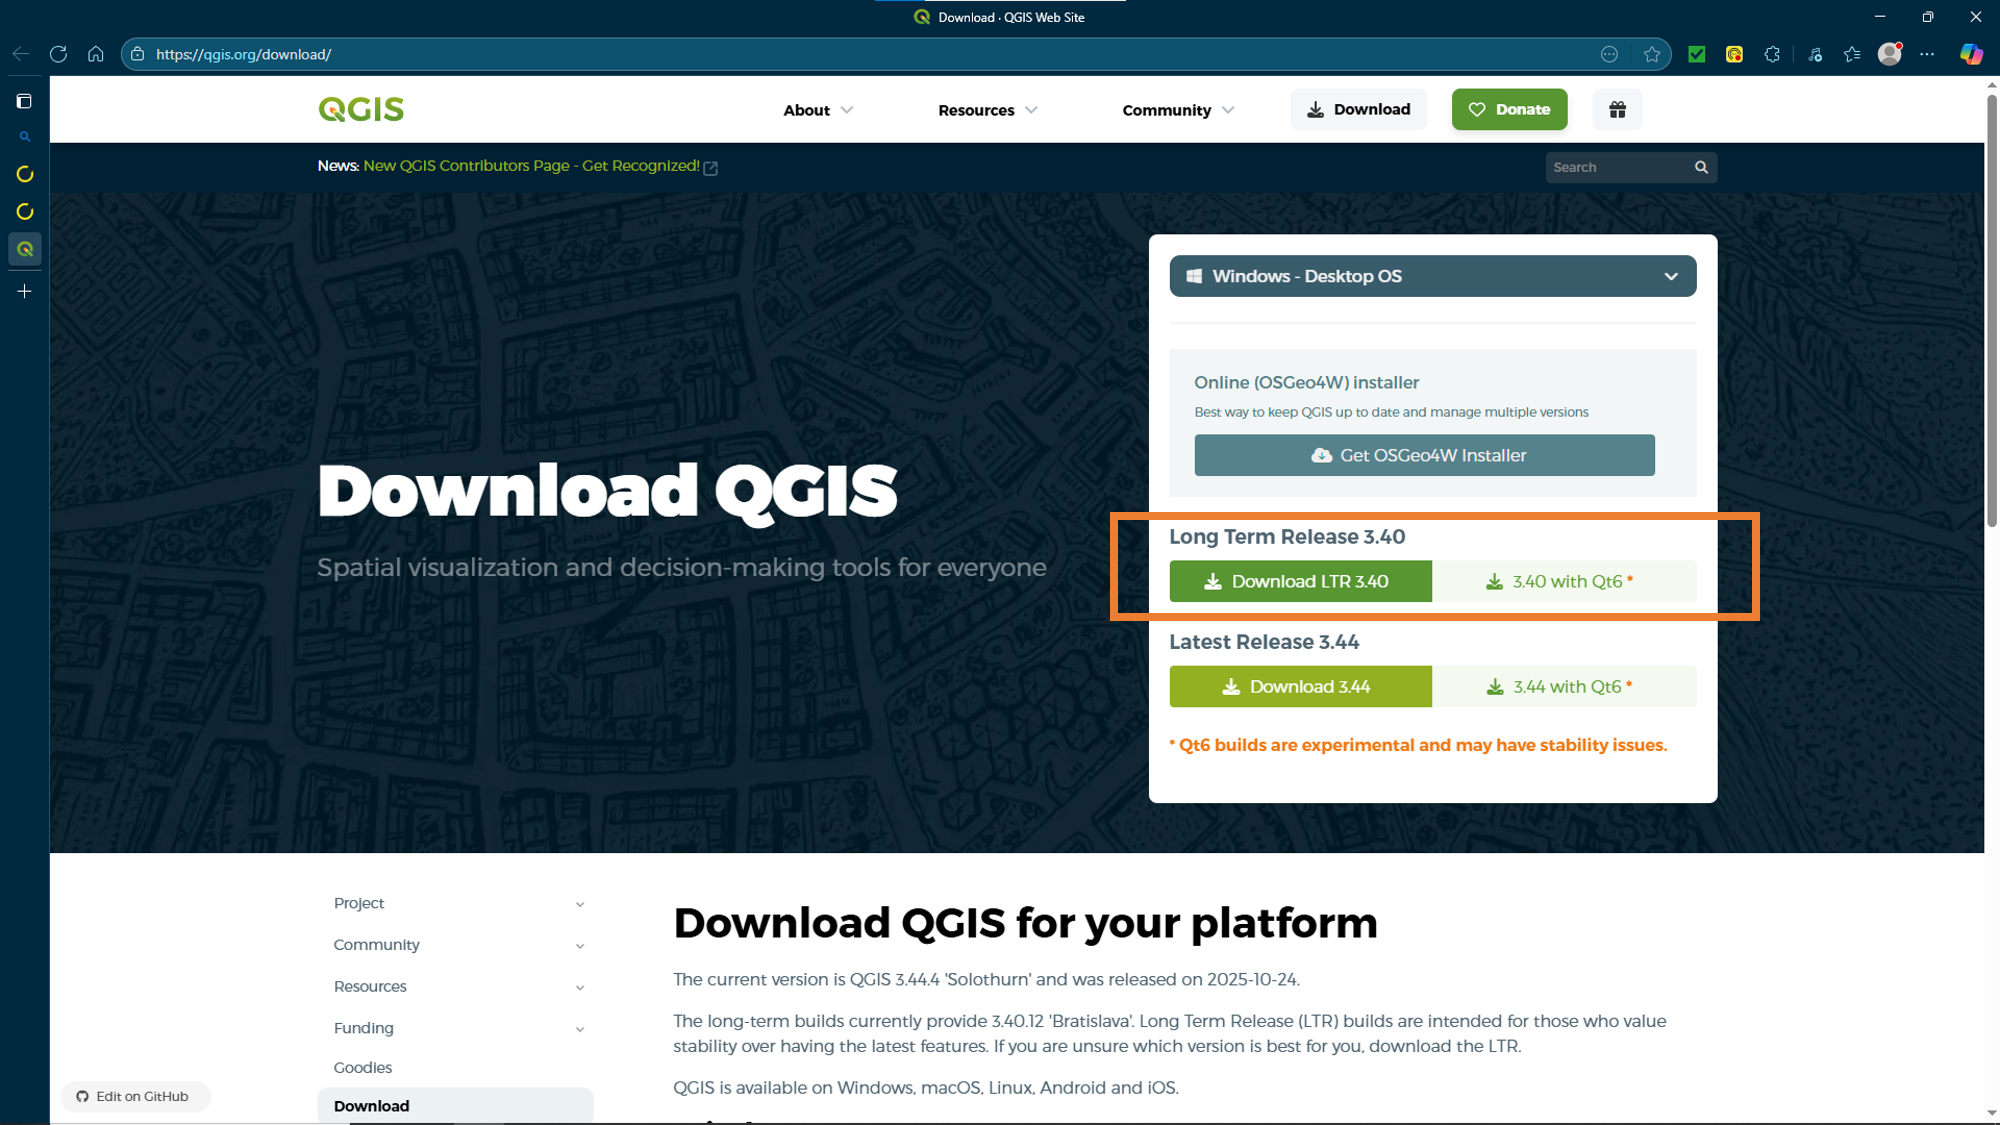
\includegraphics[width=\textwidth]{QGIS_download.png}

    We recommend downloading the {\sf Long Term Release} version, which may have a different version number than shown above.


    When working on specific projects with \qgis, we recommend creating a folder inside your project directory called, for example, \fpath{KURT_Model\0_incoming} and copying any raw project conceptual data files (e.g.\ \qgis-compatible, raster and shapefiles, \excel\ files etc.) into it, as shown here:

            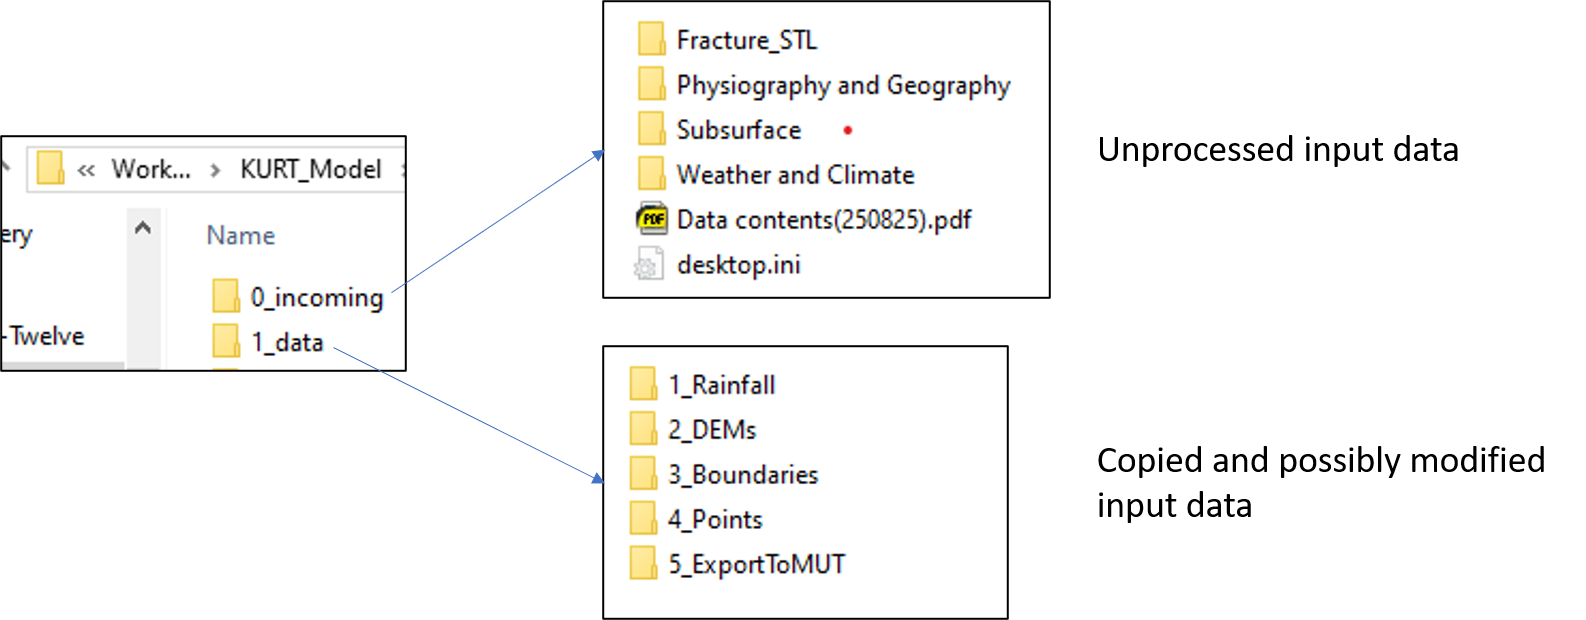
\includegraphics[width=.6\textwidth]{QGIS_FolderStructure}

    When using and modifying the data in \qgis\, we then recommend saving it in a separate working folder called, for example, \fpath{KURT_Model\1_data}

    In \qgis, we can navigate to any folder and add it to the list of favourites as a convenience:

            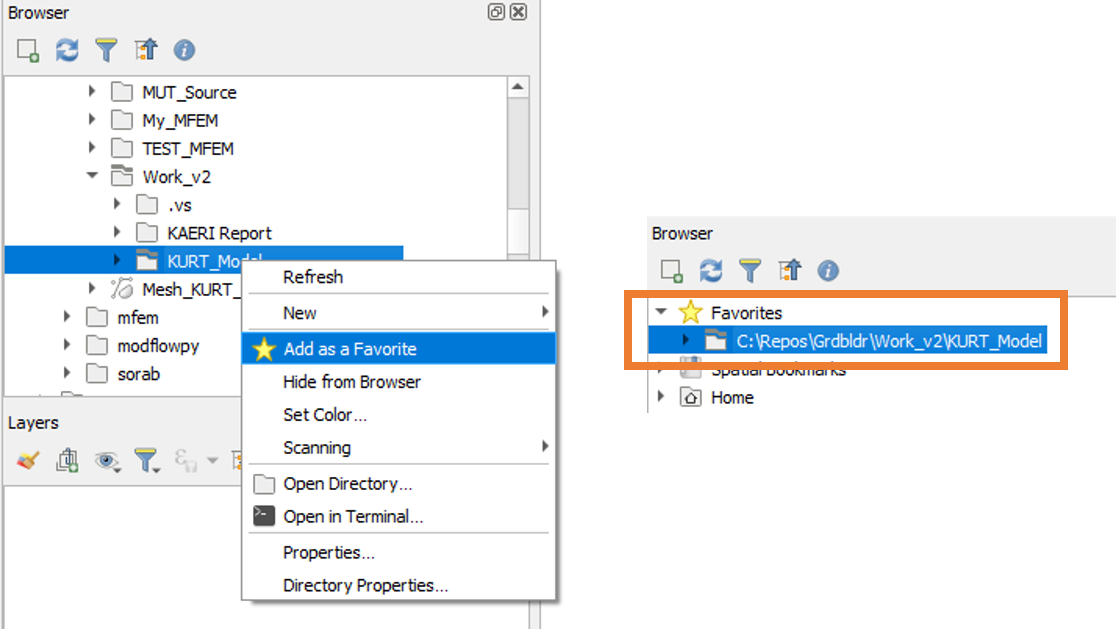
\includegraphics[width=\textwidth]{QGIS_Favourite}

    All \qgis\ project and working data files should be saved in this folder (or sub-folders contained in it) to facilitate the sharing of \qgis\ projects and their associated data.

\newpage
\section{Setting the Coordinate Reference System (CRS)}
    \label{qgis:CRS} \index{\qgis\ Usage ! Coordinate reference systems (CRS's)}
    To change the displayed units from degrees latitude and longitude to metres, apply a pre-defined Universal Transverse Mercator (UTM) projection by double-clicking the {\sf Current CRS} field to open the {\sf Project Properties - CRS} dialogue:

            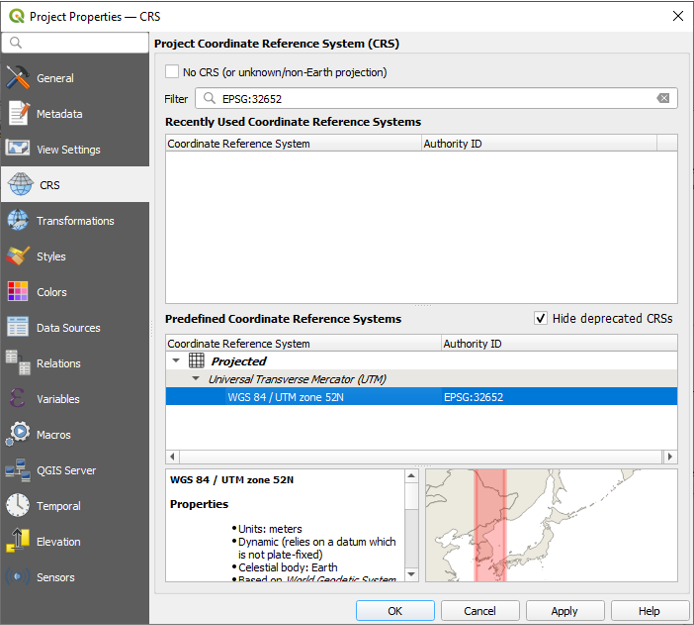
\includegraphics[width=\textwidth]{QGIS_ProjectUTM52N.png}

    In the example above the chosen projection is \texttt{EPSG:32652 - WGS 84 / UTM zone 52N}, which includes South Korea.   Initially, there may be no {\sf Recently Used Coordinate Reference Systems} to choose from so use the search field to locate it with the string, e.g.\ {\tt EPSG:32652}.  Once the desired projection is located choose it and click the {\sf Apply} button.

    Now project the DEM by choosing \menupath{Dem_all_5m.tif\Layer CRS\Set Layer CRS...} to open the dialogue or \menupath{Dem_all_5m.tif\Layer CRS\Set to EPSG:32652} if it appears in the menu:

            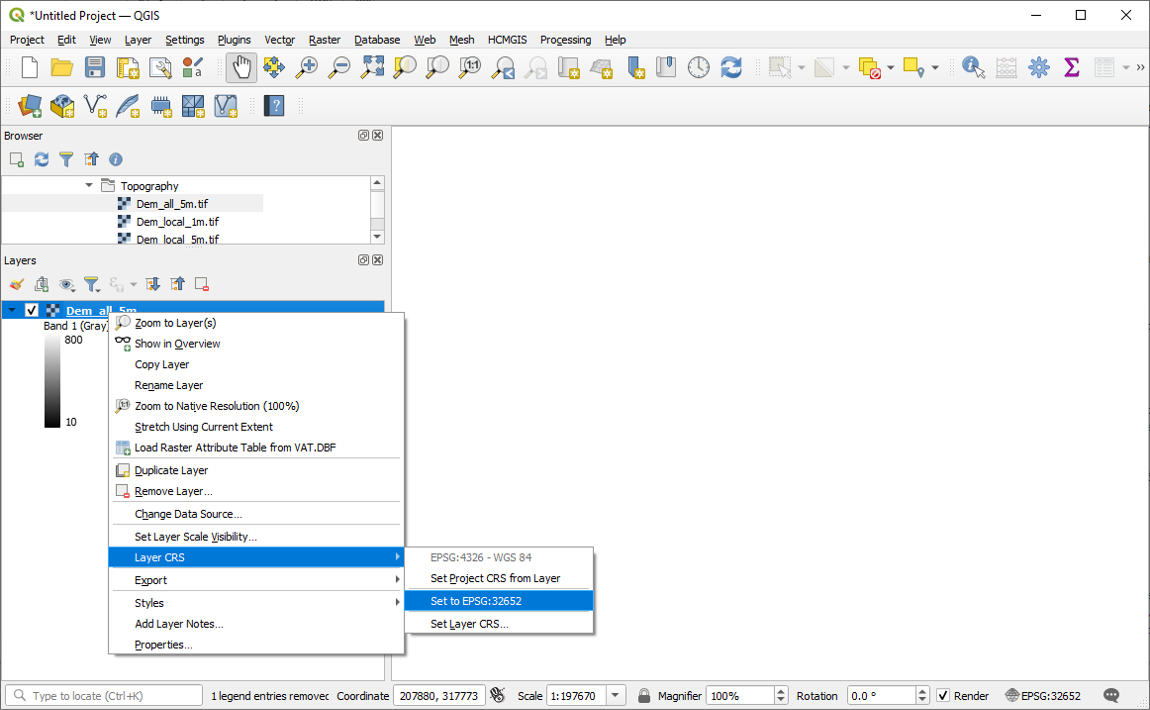
\includegraphics[width=\textwidth]{QGIS_ProjectDEM.png}

    To re-centre the DEM, choose \menupath{Dem_all_5m.tif\Zoom to Layer(s)}. Note that the displayed coordinates are now in metres.

\newpage
\section{Layers}

    \subsection{Layer Properties}
        \label{qgis:DEM_Properties} \index{\qgis\ Usage ! Layer properties}
        The layer  properties dialogue can be opened by double-clicking on the layer name or by right-clicking and choosing {\sf Properties} from the drop-down menu:\footnote{Note that detailed documentation for \qgis\ tools is often available through the {\sf Help} button in the lower right corner of the dialogue.}

                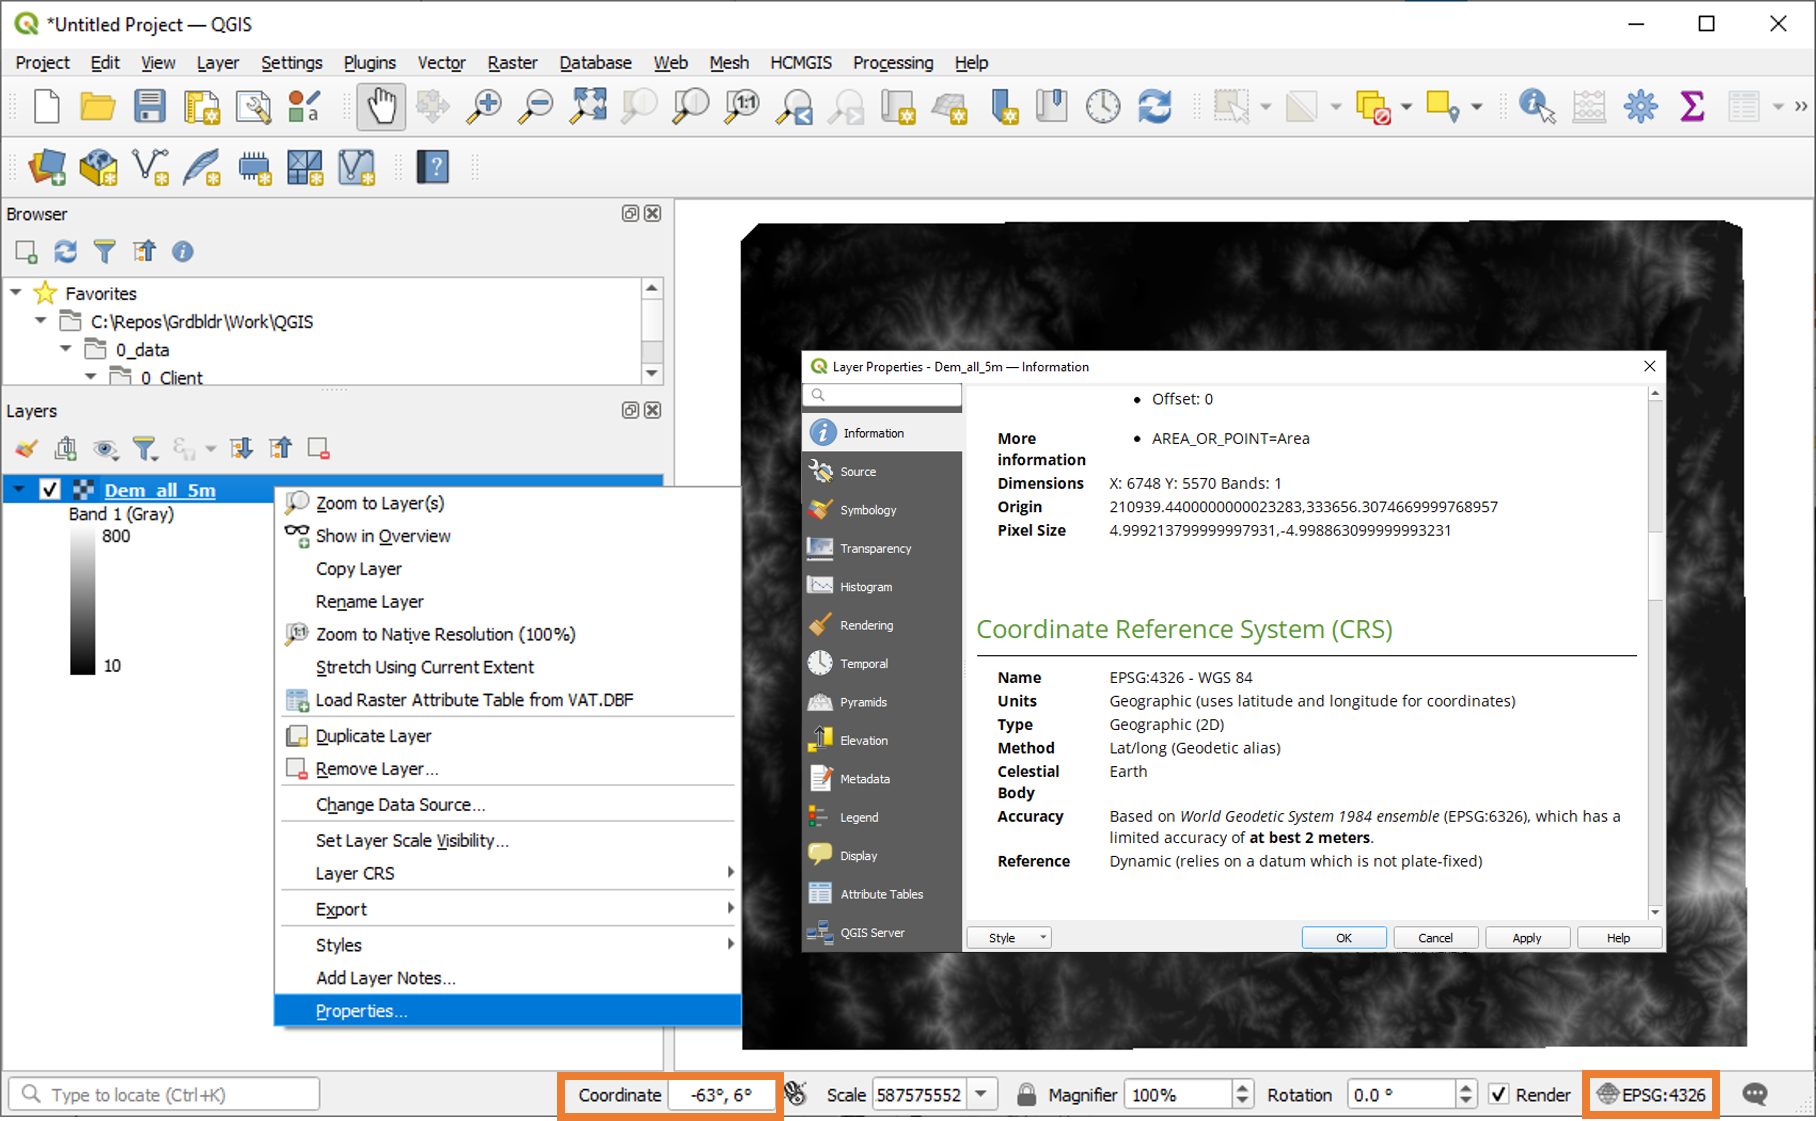
\includegraphics[width=\textwidth]{QGIS_DEMPropertiesLatLong}

        Note the following in the example shown above:
        \begin{itemize}
        \item Properties for the raster layer layer {\sf Dem\_all\_5m} are being viewed.
        \item The raster has a pixel size of about 5-by-5-metres
        \item The Coordinate Reference System (CRS) is in units of degrees latitude and longitude.
        \item The {\sf Current CRS}  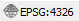
\includegraphics[height=0.7\baselineskip]{Button_CurrentCRS} is shown in the lower right hand corner of the \qgis\ window.
        \end{itemize}


    \newpage
    \subsection{Layer Appearance (symbology)}
        \label{qgis:symbology} \index{\qgis\ Usage ! Layer appearance (symbology)}
        The layer symbology dialogue can be opened by double-clicking on the layer name or by right-clicking and choosing {\sf Properties} from the drop-down menu:

                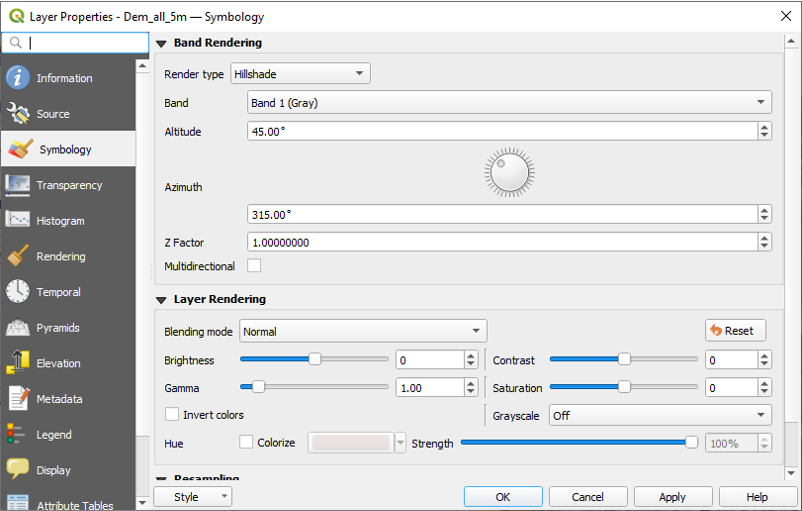
\includegraphics[width=\textwidth]{QGIS_DEMPropertiesSymbology}

        In the example above we have chosen {\sf Render Type - Hillshade} for the raster layer \menupath{Dem_all_5m.tif\Properties\Symbology}.


    \newpage
    \subsection{Layer Clipping}
        \label{qgis:clip} \index{\qgis\ Usage ! Clipping a layer}
        Once the extents of the model domain have been determined, the DEM can be clipped to a smaller size which saves disk space. Clip the raster by choosing (\menupath{Raster\Extraction\Clip by extent}) and then the \menupath{Clipping extent option\Draw on Map Canvas}.  The mouse cursor will be shown as a 'plus' sign. Click and drag a rectangle delimiting the area to take into account, in this case enclosing the regional boundary.  The resulting clipped rectangular region is shown below as a hillshade inside the original unclipped DEM.

            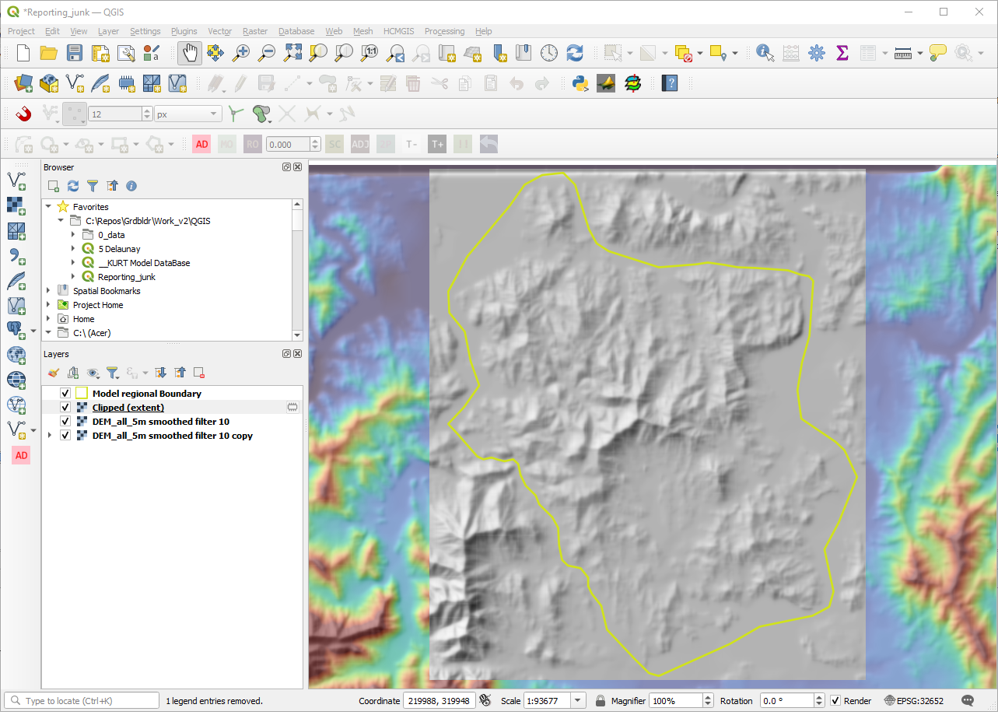
\includegraphics[width=\textwidth]{QGIS_ClippedDem}


    \newpage
    \subsection{Vector Layers}
        \subsubsection{Loading Vector Layers}
            To load a vector layer, simply drag and drop the vector file into the \qgis\ workspace:
            \label{qgis:LoadVector} \index{\qgis\ Usage ! Loading a vector layer}

        \newpage
        \subsubsection{Selecting Features}
            \label{qgis:SelectFeatures} \index{\qgis\ Usage ! Selecting features}
            In \qgis\, features can be selected using the {\sf Selection Toolbar}, shown below in the orange box:

                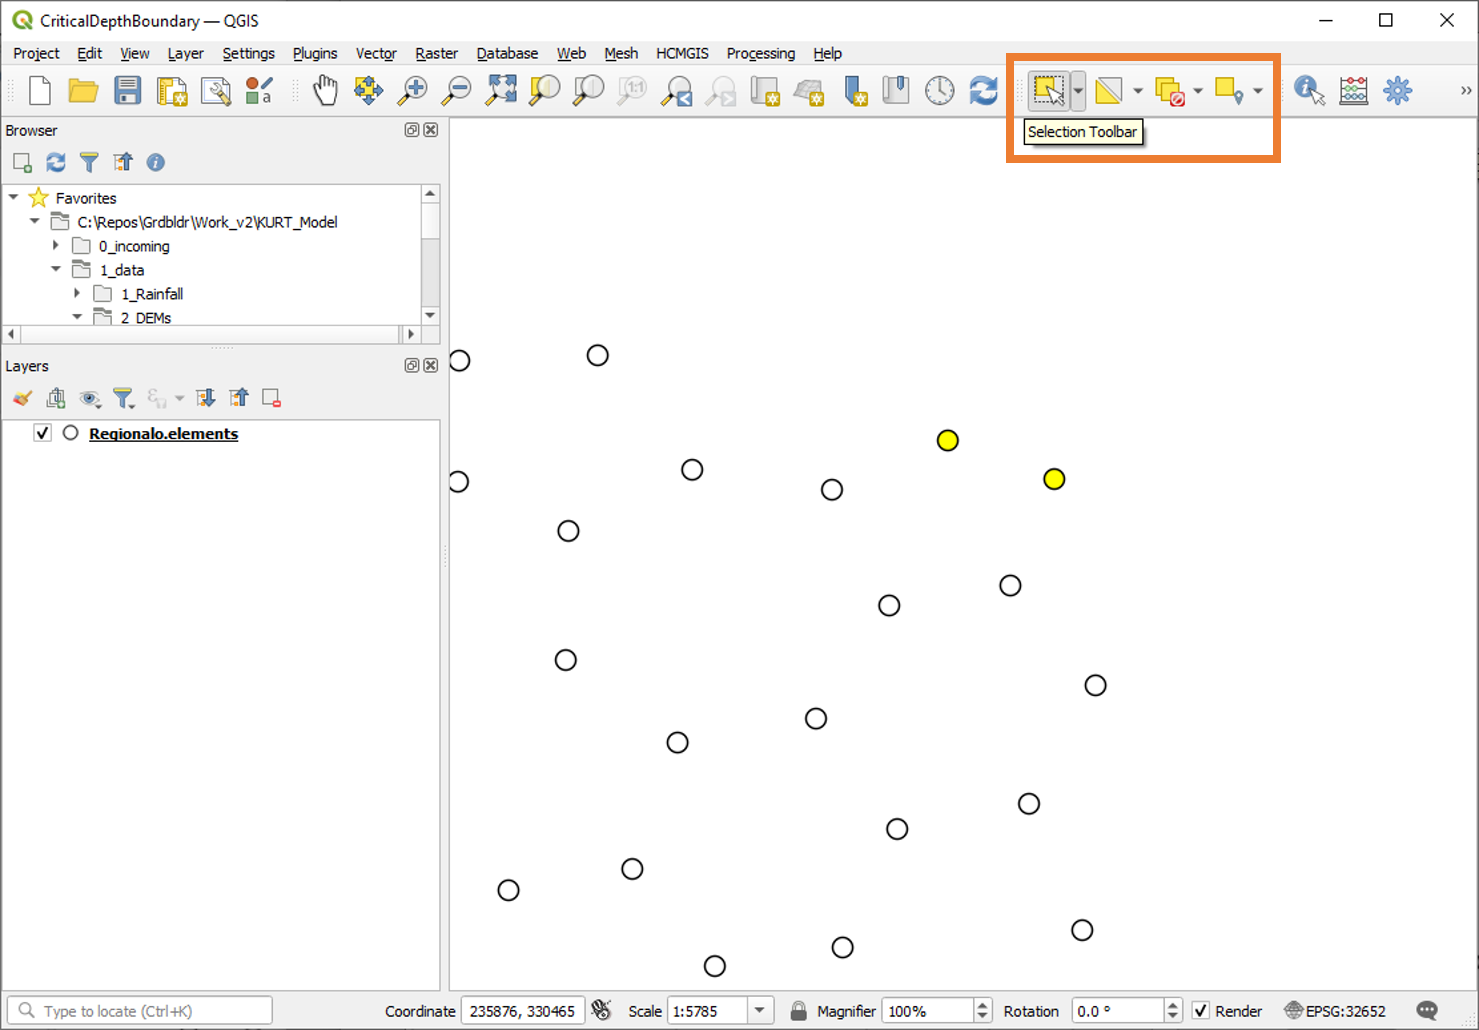
\includegraphics[width=0.9\textwidth]{QGIS_SelectFeatures.png}

             In this example, we are using the option {\sf Select features by area or single click} 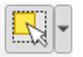
\includegraphics{QGIS_SelectFeaturesButton.png} to choose points (white circles) in a vector layer called {\sf Regionalo.elements}.  The currently selected points are shown here as yellow-highlighted circles.  To choose multiple points, hold down the {\tt shift} key while left-clicking on the feature.


        \newpage
        \subsubsection{Extract Vertices}
            \label{qgis:ExtractVertices} \index{\qgis\ Usage ! Extract vertices}
            In \qgis\, vertices can be extracted from an active vector layer by choosing \menupath{Vector\Geometry Tools\Extract Vertices} as shown below:

                    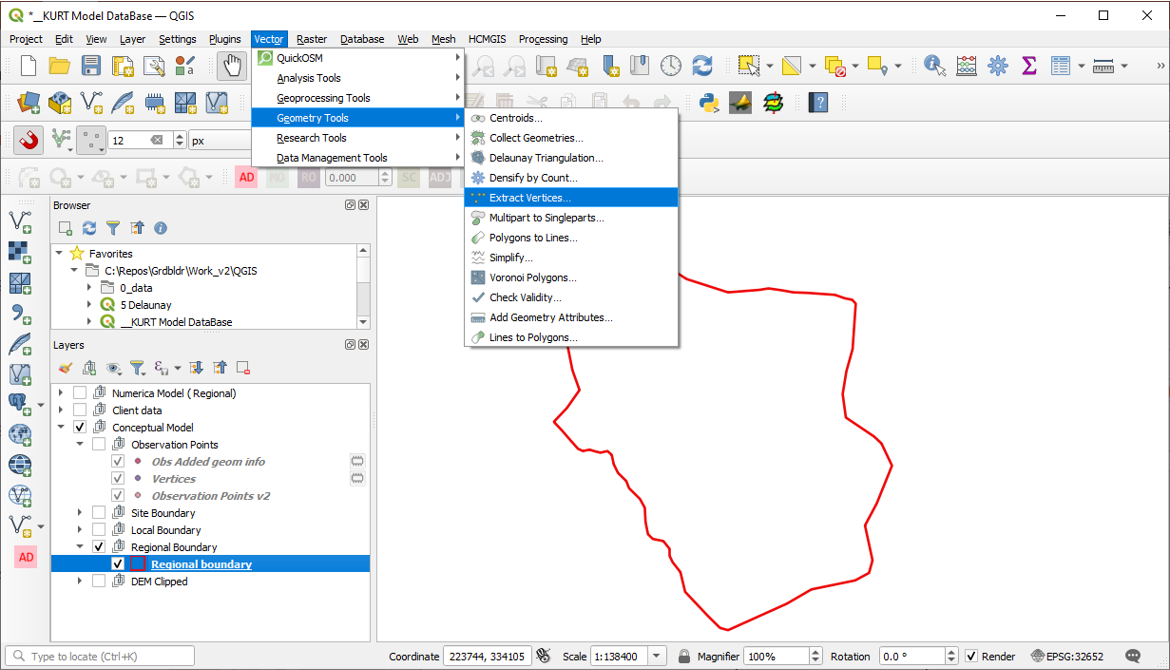
\includegraphics[width=0.9\textwidth]{QGIS_ExportVertices_1.png}

            This opens the {\sf Extract Vertices} dialogue:

                    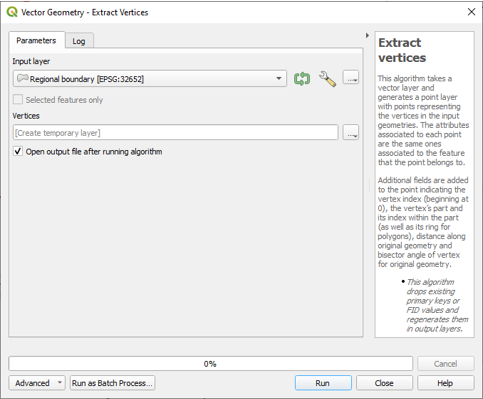
\includegraphics[width=0.6\textwidth]{QGIS_ExportVertices_2.png}

            The active layer, in this case {\sf Regional Boundary}, is shown in the {\sf Input layer} field and can be changed if desired. Choose {\sf Run}.

            This creates a new layer called {\sf Vertices}, and adds vertex locations along the local boundary as shown here by the pink circles:

                    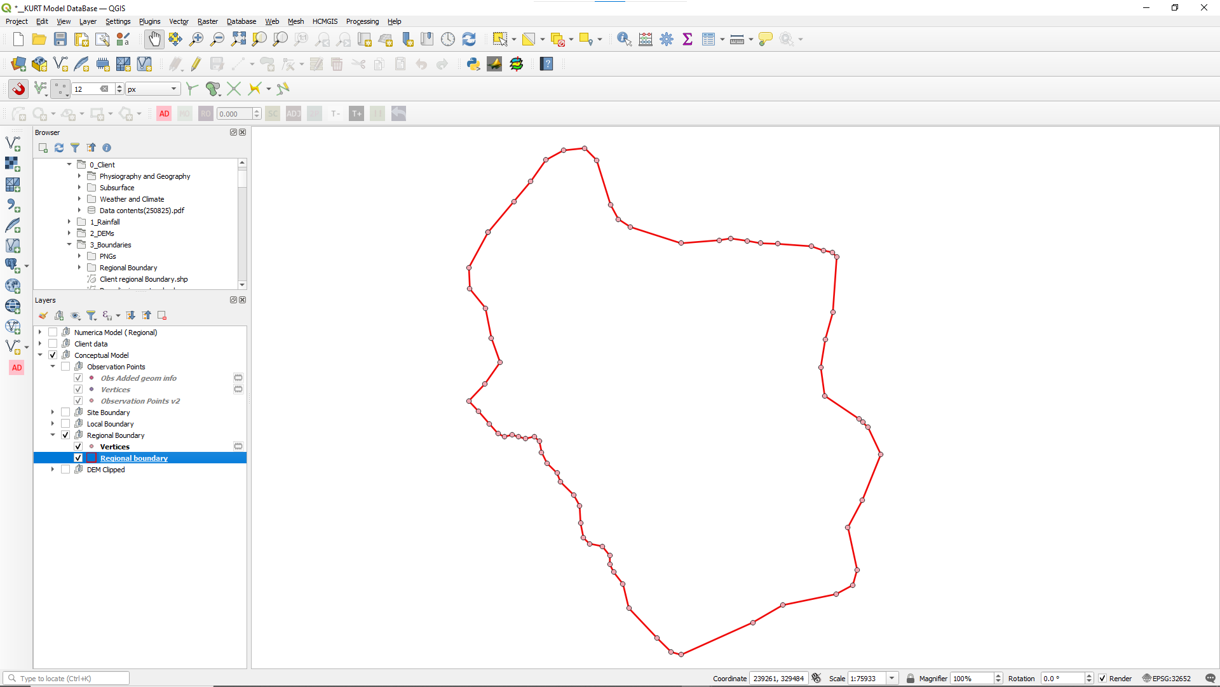
\includegraphics[width=0.9\textwidth]{QGIS_ExportVertices_3.png}

            Right-click on the {\sf vertices} layer and choose {\sf Open Attribute Table} as shown below:

                    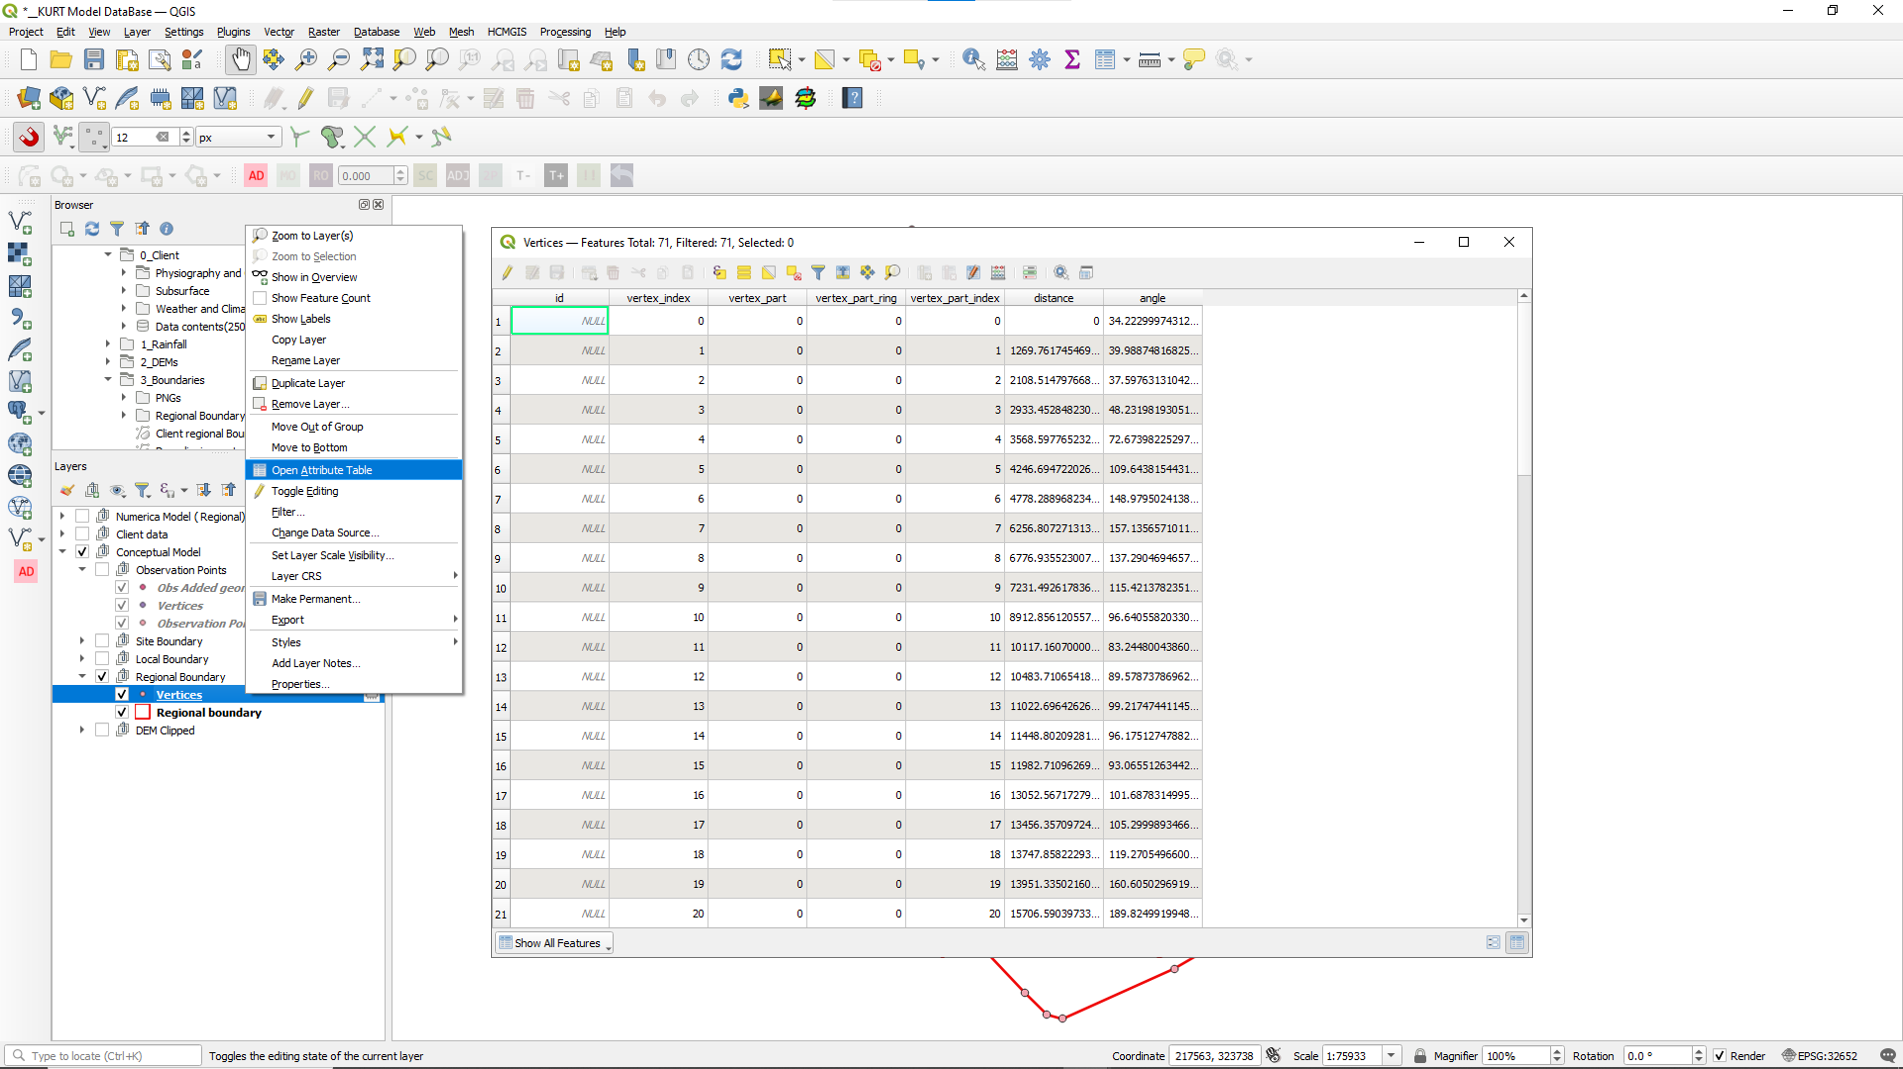
\includegraphics[width=0.9\textwidth]{QGIS_ExportVertices_4.png}

            In this example, the table contains the {\sf distance} and {\sf angle}  from {\sf vertex\_index} $0$ to the other vertices in the polygon.

        \newpage
        \subsubsection{Add Geometry Attributes}
            \label{qgis:AddGeometryAttributes} \index{\qgis\ Usage ! Add geometry attributes}
            Geometry attributes (e.g.\ $xy$ coordinates, Delaunay triangle vertice id's) can be extracted from an active vector layer by choosing \menupath{Vector\Geometry Tools\Add geometry attributes...} as shown below:

                    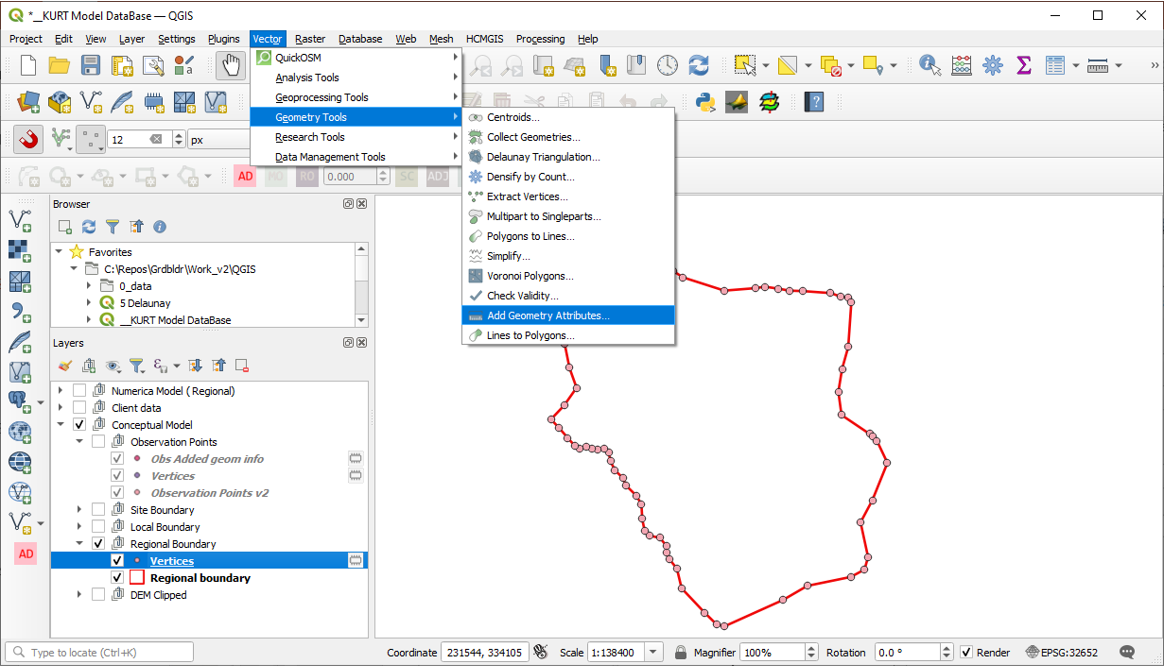
\includegraphics[width=0.9\textwidth]{qgis_AddGeometryAttributes_1.png}

            This opens the {\sf Add Geometry Attributes} dialogue:

                    \includegraphics[width=0.6\textwidth]{qgis_AddGeometryAttributes_2.png}

            The active layer, in this case {\sf vertices}, is shown in the {\sf Input layer} field. Choose {\sf Run}.

            This creates a new layer called {\sf Added geom info}, and adds vertex locations along the local boundary as shown here by the purple circles:

                    \includegraphics[width=0.9\textwidth]{qgis_AddGeometryAttributes_3.png}

            Right-click on the {\sf Added geom info} layer and choose {\sf Open Attribute Table} to see the table shown below:

                    \includegraphics[width=0.9\textwidth]{qgis_AddGeometryAttributes_4.png}

            In this example, the table has two additional columns {\sf xcoord} and {\sf ycoord} containing the $x$ and $y$ coordinates respectively.

        \newpage
        \subsubsection{Georeference an Image}
            \label{qgis:Georeference}  \index{\qgis\ Usage ! Georeference an image}

            This image can be imported into \qgis\ using the {\sf Freehand Raster Georeferencer} plugin, which is installed using \menupath{Plugin\Manage and Install Plugins}, as shown below:

                    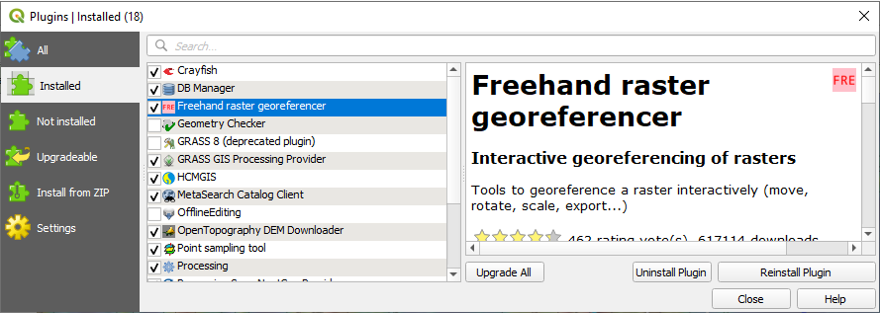
\includegraphics[width=0.7\textwidth]{QGIS_FreehandPlugin.png}

            Once installed, make sure the plugin toolbar is visible by choosing \menupath{View\Panels\Freehand Raster Georeferencer}.  To import the regional boundary image file, click the {\sf AD} button as shown below left and choose the file shown in the browser window below right:

                    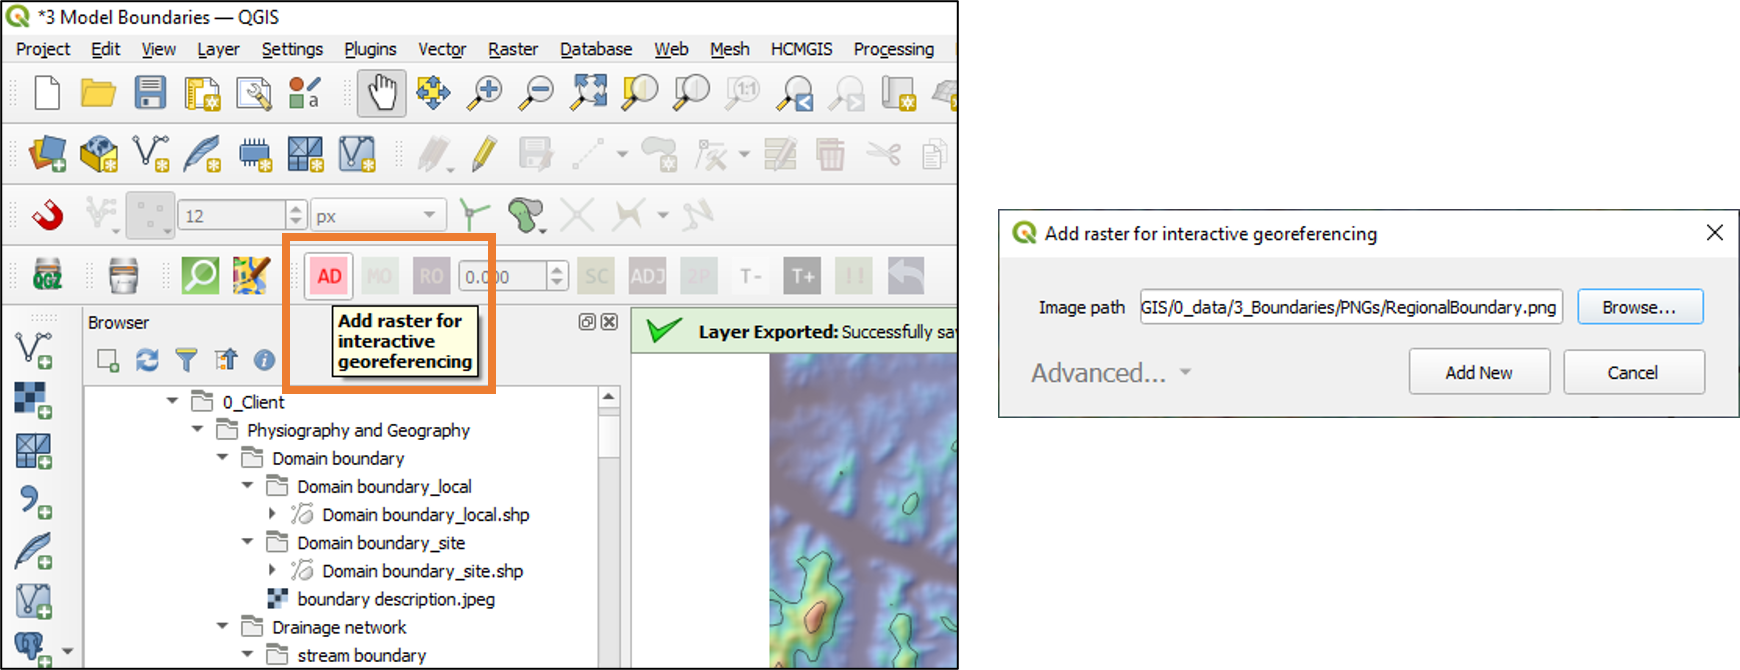
\includegraphics[width=0.9\textwidth]{QGIS_load_reg_png}

            Below we see the imported image superimposed over the \qgis\ workspace.

                    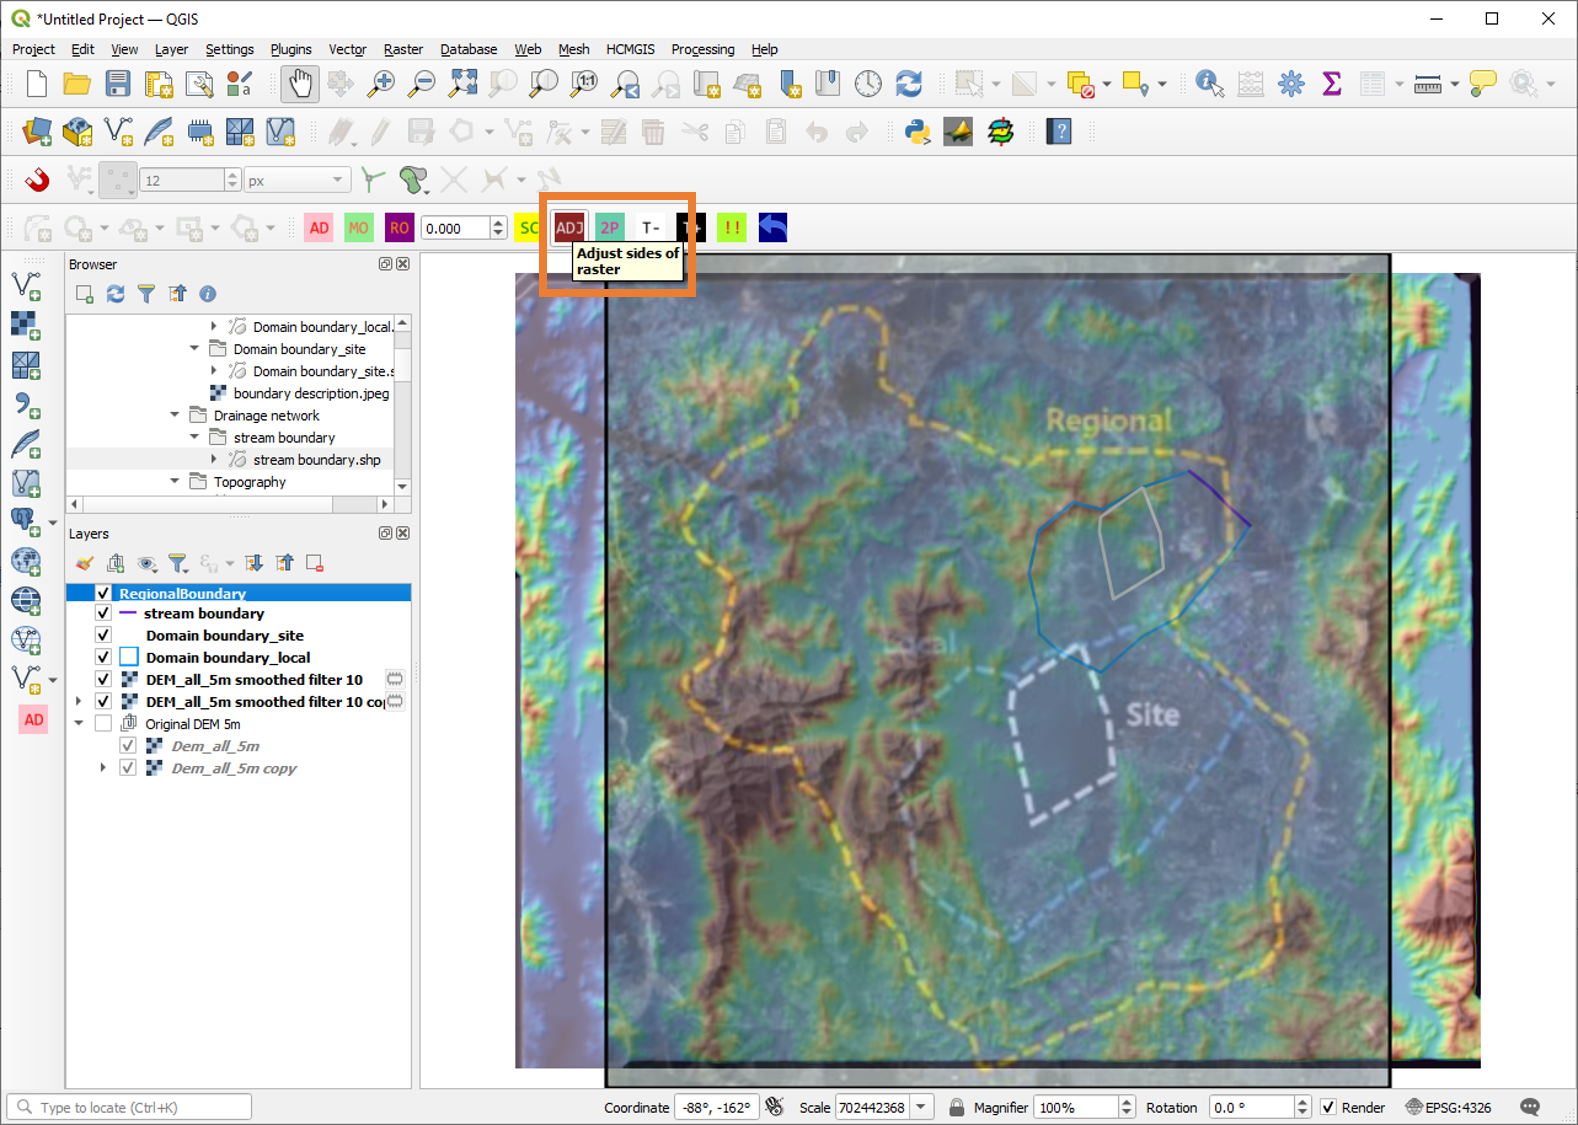
\includegraphics[width=0.9\textwidth]{QGIS_adjust_reg_png}

            Note that the image boundaries are not lined up with the local and site shapefile boundaries.

            Use the {\sf ADJ} button to move the sides of the image around until the boundaries are aligned as shown below:

                    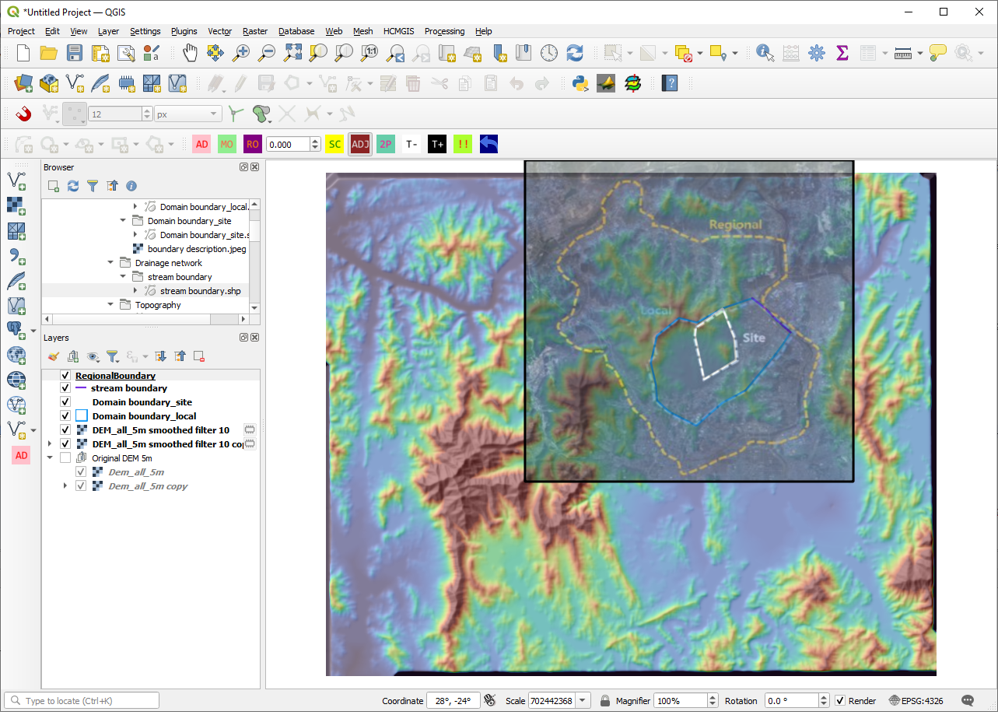
\includegraphics[width=0.9\textwidth]{QGIS_adjusted_reg_png}

        \newpage
        \subsubsection{Add a new shapefile}
            \label{qgis:AddNewShapefile}  \index{\qgis\ Usage ! Add a new shapefile}
            If the Manage Layers Toolbar is not visible,choose \menupath{View\Panels\Manage Layers Toolbar}.  To create a new shapefile, choose the {\sf New Shapefile Layer...} button 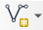
\includegraphics[height=0.7\baselineskip]{Button_NewShapefileLayer} to open the dialogue shown below:

                    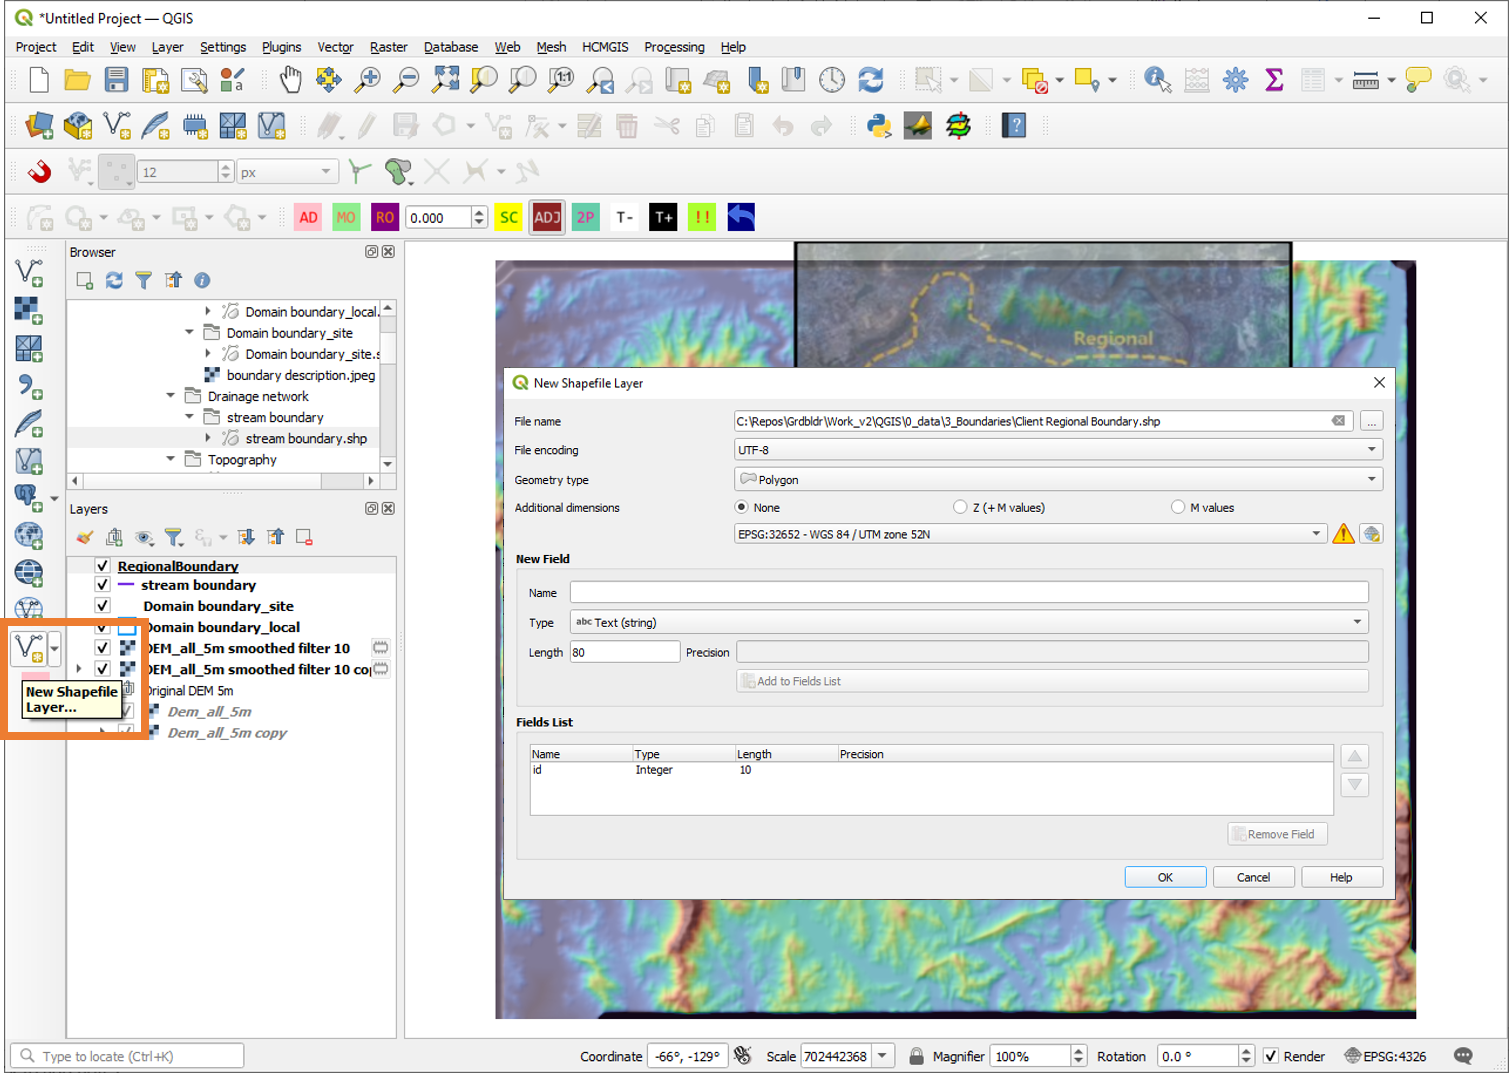
\includegraphics[width=0.9\textwidth]{QGIS_AddNewShapefile.png}


            In this example, the {\sf Geometry type} is set to {\sf Polygon}, the project CRS to  {\sf EPSG:32652 - WGS 84 / UTM zone 52N} and the shapefile name is {\sf Client Regional Boundary}.

            In the example below, a shapefile suitable for storing  e.g.\ observation point data is defined:

                    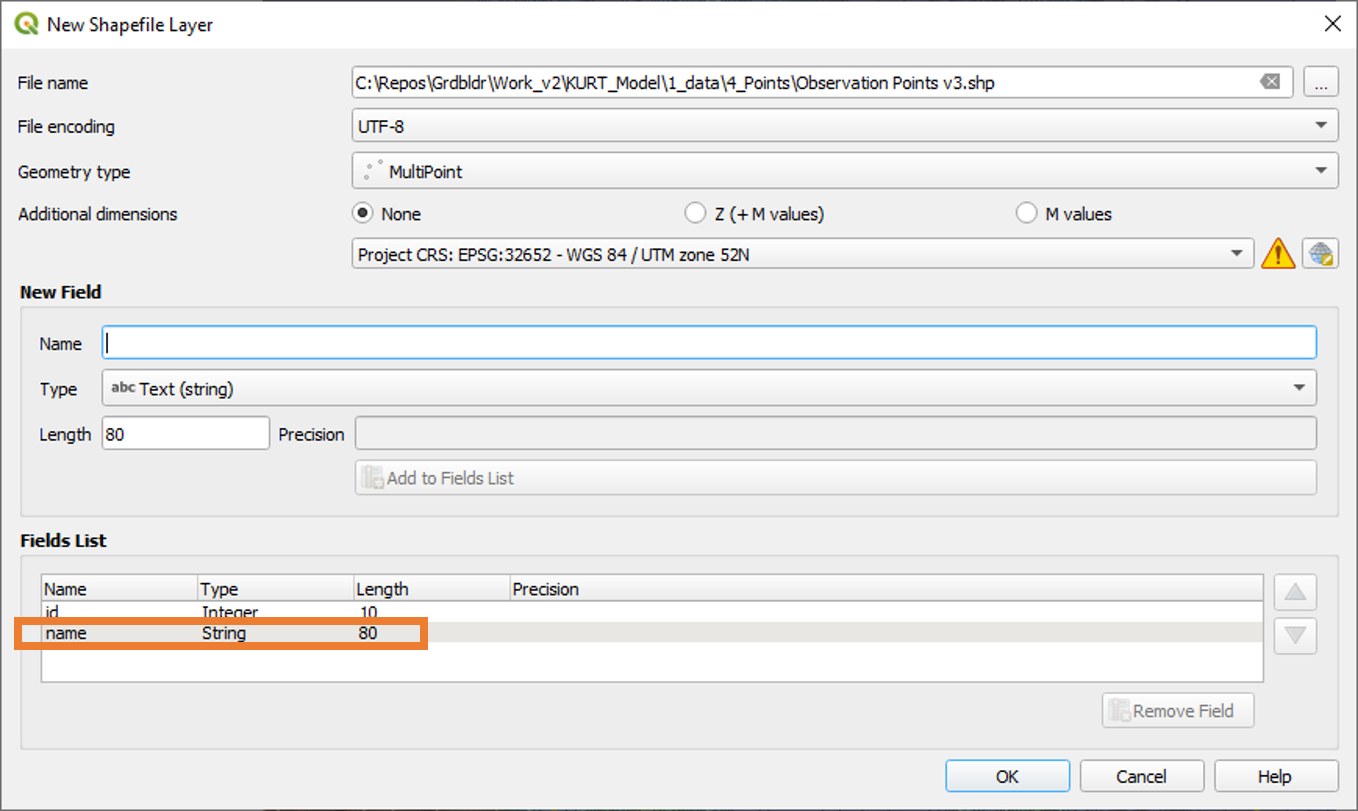
\includegraphics[width=0.9\textwidth]{QGIS_AddNewShapefile_points.png}

            Here the {\sf Geometry type} is set to {\sf Multipoint} and the shapefile name is {\sf Observation Points v3}.  A new field called {\tt name} has been defined to store the observation point names of type string.


        \newpage
        \subsubsection{Digitize a new shapefile}
            \label{qgis:DigitizeNewShapefile}  \index{\qgis\ Usage ! Digitize a new shapefile}
            If the digitizing toolbar is not visible, choose \menupath{View\Panels\Digitizing toolbar}.  To start digitizing choose the {\sf Toggle Editing} button 
\includegraphics[height=0.7\baselineskip]{Button_ToggleEditting}, then the {\sf Add Polygon Feature} button 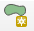
\includegraphics[height=0.7\baselineskip]{Button_AddPolygonFeature}.  The mouse cursor should now be shown as a crosshair.  Move the crosshair to a point on the regional boundary and click the left-mouse button to digitize a new boundary point.  The example below shows a partially digitized polygon:

                    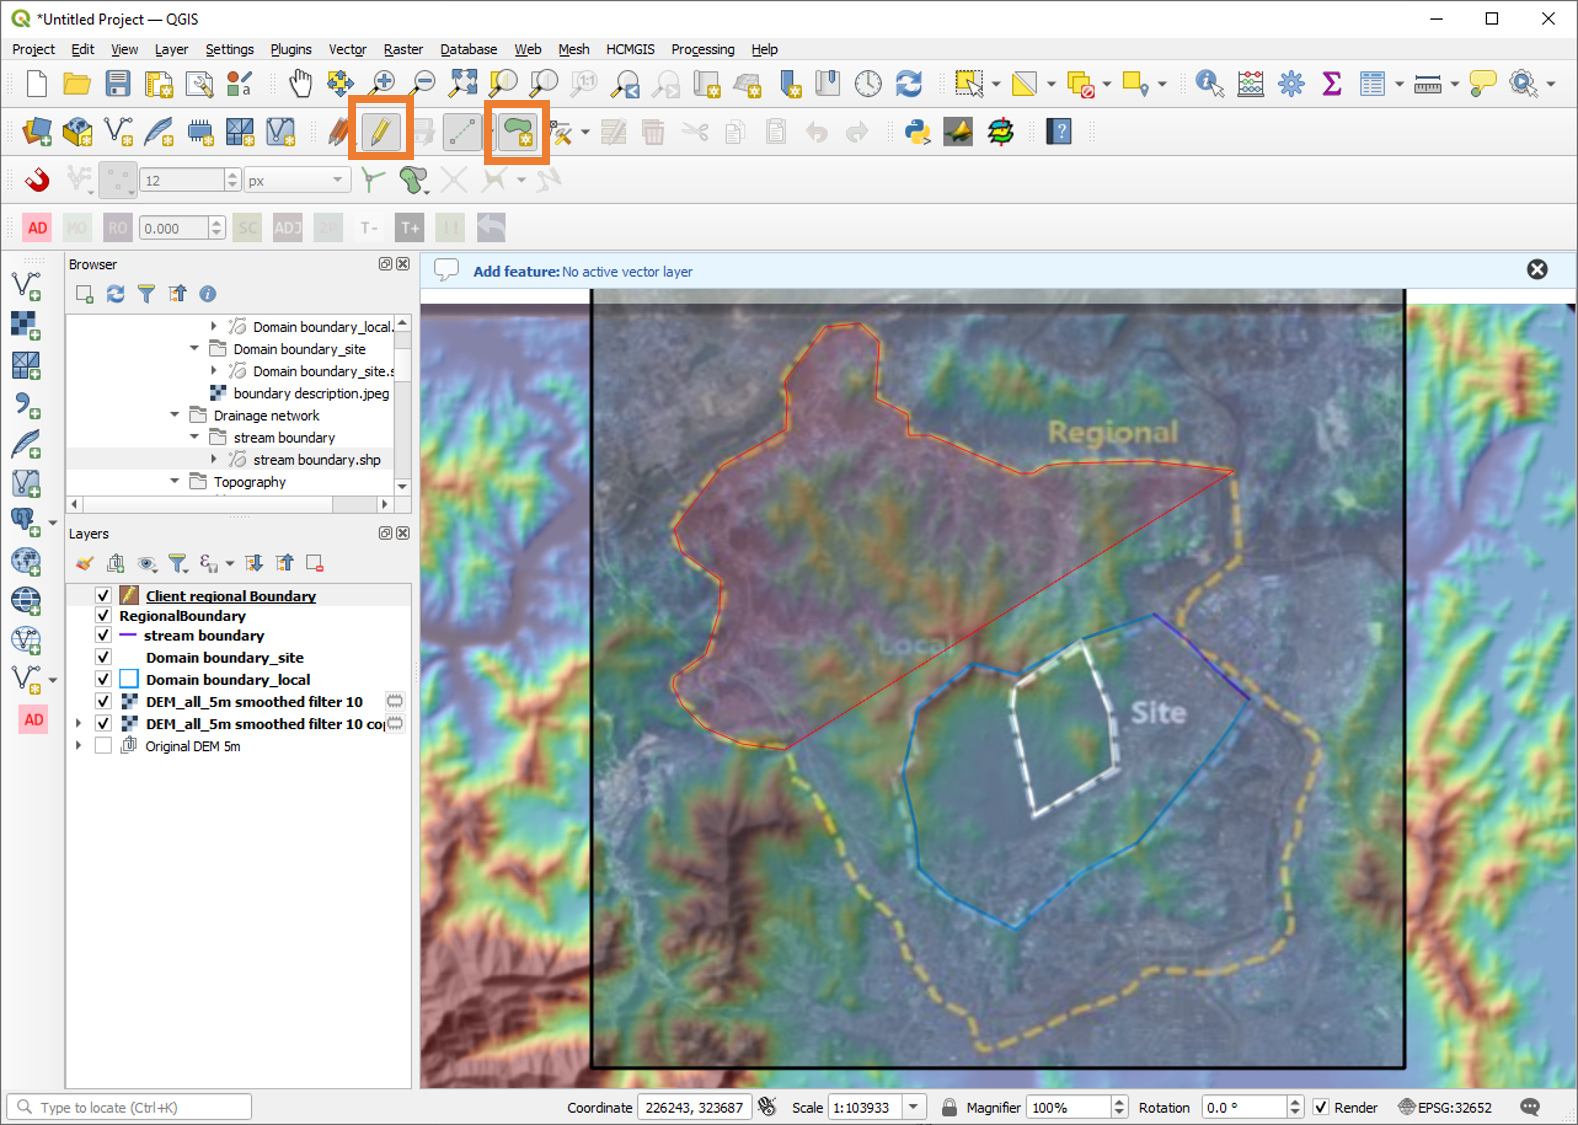
\includegraphics[width=0.9\textwidth]{QGIS_DigitizingNewShapefile}

            Proceed around the polygon boundary, left-clicking the mouse to define new polygon vertices, and finally right-clicking the mouse to close it.
        \newpage
        \subsubsection{Point Sampling From a Raster Layer}
            \label{qgis:PointSamplingTool} \index{\qgis\ Usage ! Point sampling tool}
            The {\sf PointSamplingTool} can be used to map elevations from a raster layer (i.e.\ a DEM) to the vertices of a vector layer. This plugin may need to be installed using \menupath{Plugin\Manage and Install Plugins}, as shown below:

                    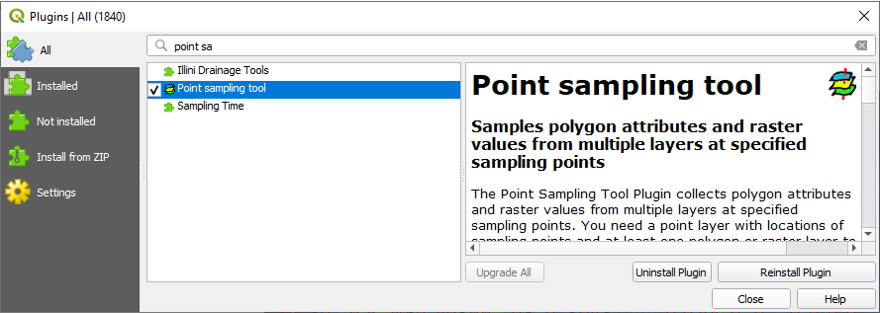
\includegraphics[width=\textwidth]{QGIS_PointSamplingToolPlugin_1.png}

            Once installed, the {\sf Point sampling tool} button 
\includegraphics[height=0.7\baselineskip]{QGIS_PointSamplingToolIcon.png} should appear in the {\sf Plugins toolbar}.

            First, activate the layer, then click on {\sf Point sampling tool} button 
\includegraphics[height=0.7\baselineskip]{QGIS_PointSamplingToolIcon.png} to open the {\sf Point Sampling Tool} dialogue shown below:

                    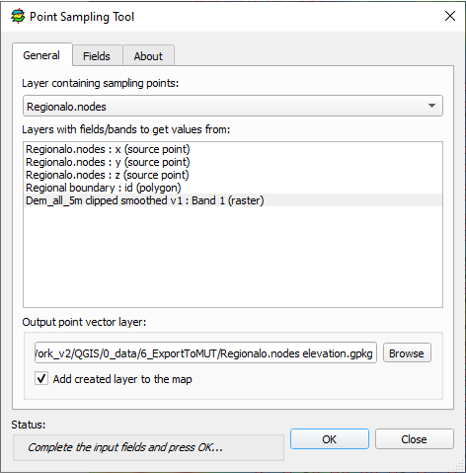
\includegraphics[width=0.6\textwidth]{QGIS_PointSamplingToolPlugin_2.png}

            In this example the field {\sf Layer containing sampling points:} is referring to a vector layer of points {\sf Regionalo.nodes}.

            The field {\sf Layers with fields/bands to get values from:} contains a list of vector and raster layers available to sample from.  Click on a layer to choose it and it will be indicated with a light gray shading. In this case the layer {\sf Dem\_all\_5m clipped smoothed v1: Band 1 (raster)} is the only one chosen.

            The field {\sf Output point vector layer:} contains the full path and name of the file to store the sampled elevations in. Click the {\sf Ok} button to do the sampling and then close the dialogue.

            This creates a new layer called {\sf Regionalo.nodes elevation.gpkg}.  Right-click on it and choose {\sf Open Attribute Table}, which is shown below:

                    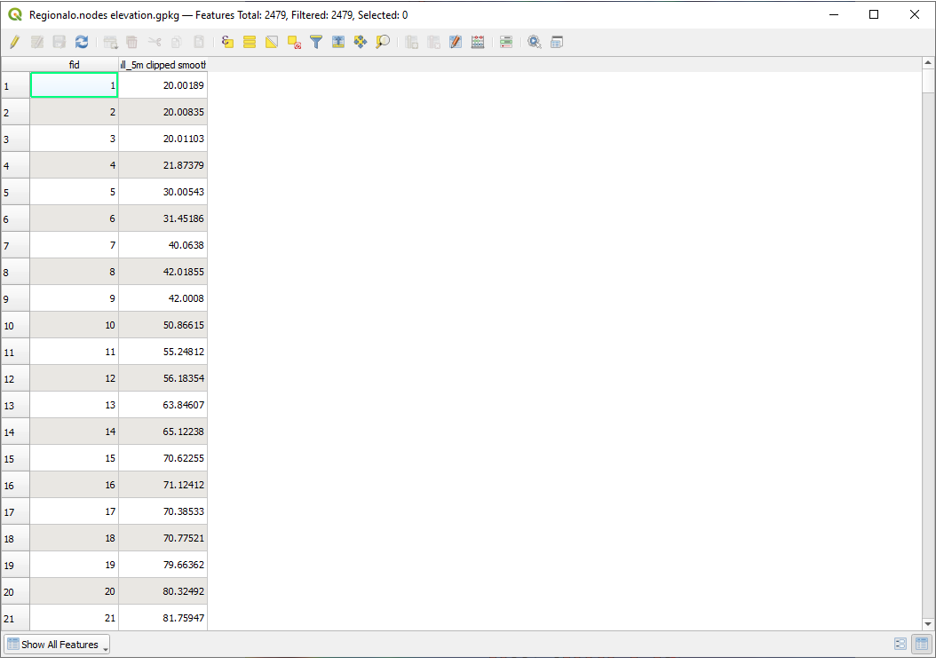
\includegraphics[width=\textwidth]{QGIS_PointSamplingToolPlugin_3.png}

            This is the list of sampled elevations, one for each point in the layer {\sf Regionalo.nodes}.


        \newpage
        \subsubsection{Export to a CSV File}
            \label{qgis:ExportToCSVFile} \index{\qgis\ Usage ! Export to a CSV file}
            The attribute table of an active vector layer can be exported to a {\tt CSV} file by right-clicking on the vector name and choosing \menupath{Export\Save features as...} as shown below:

                    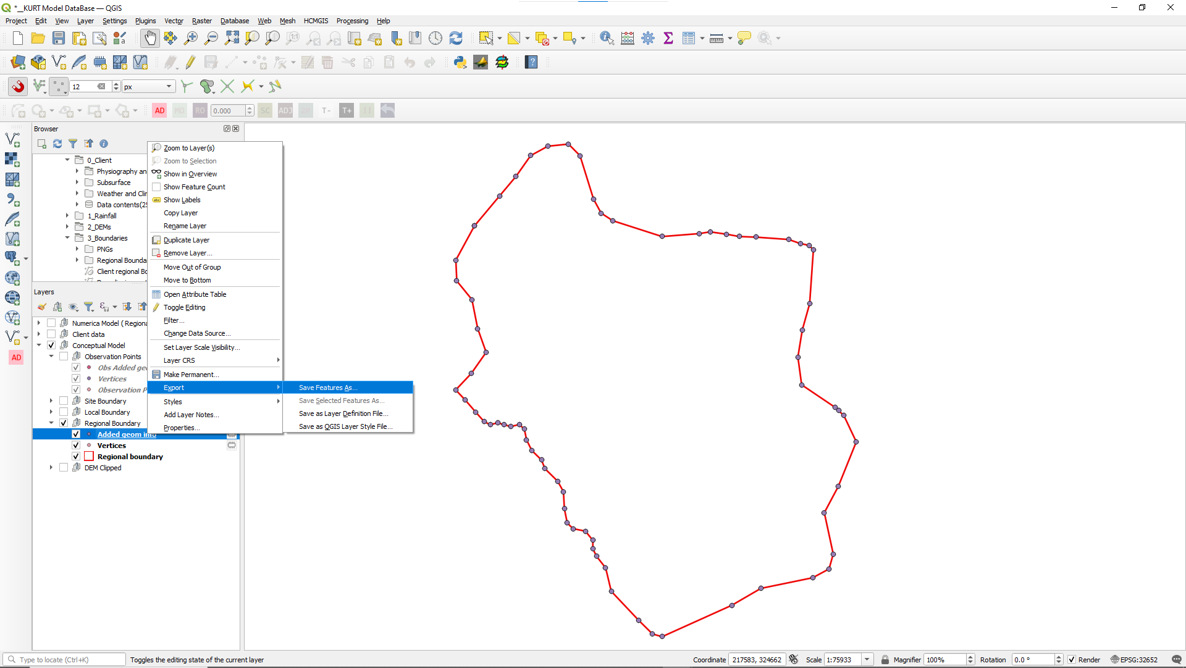
\includegraphics[width=0.9\textwidth]{QGIS_ExportToCSVFile_1.png}

            This opens the {\sf Save Features as} dialogue shown below left:

                    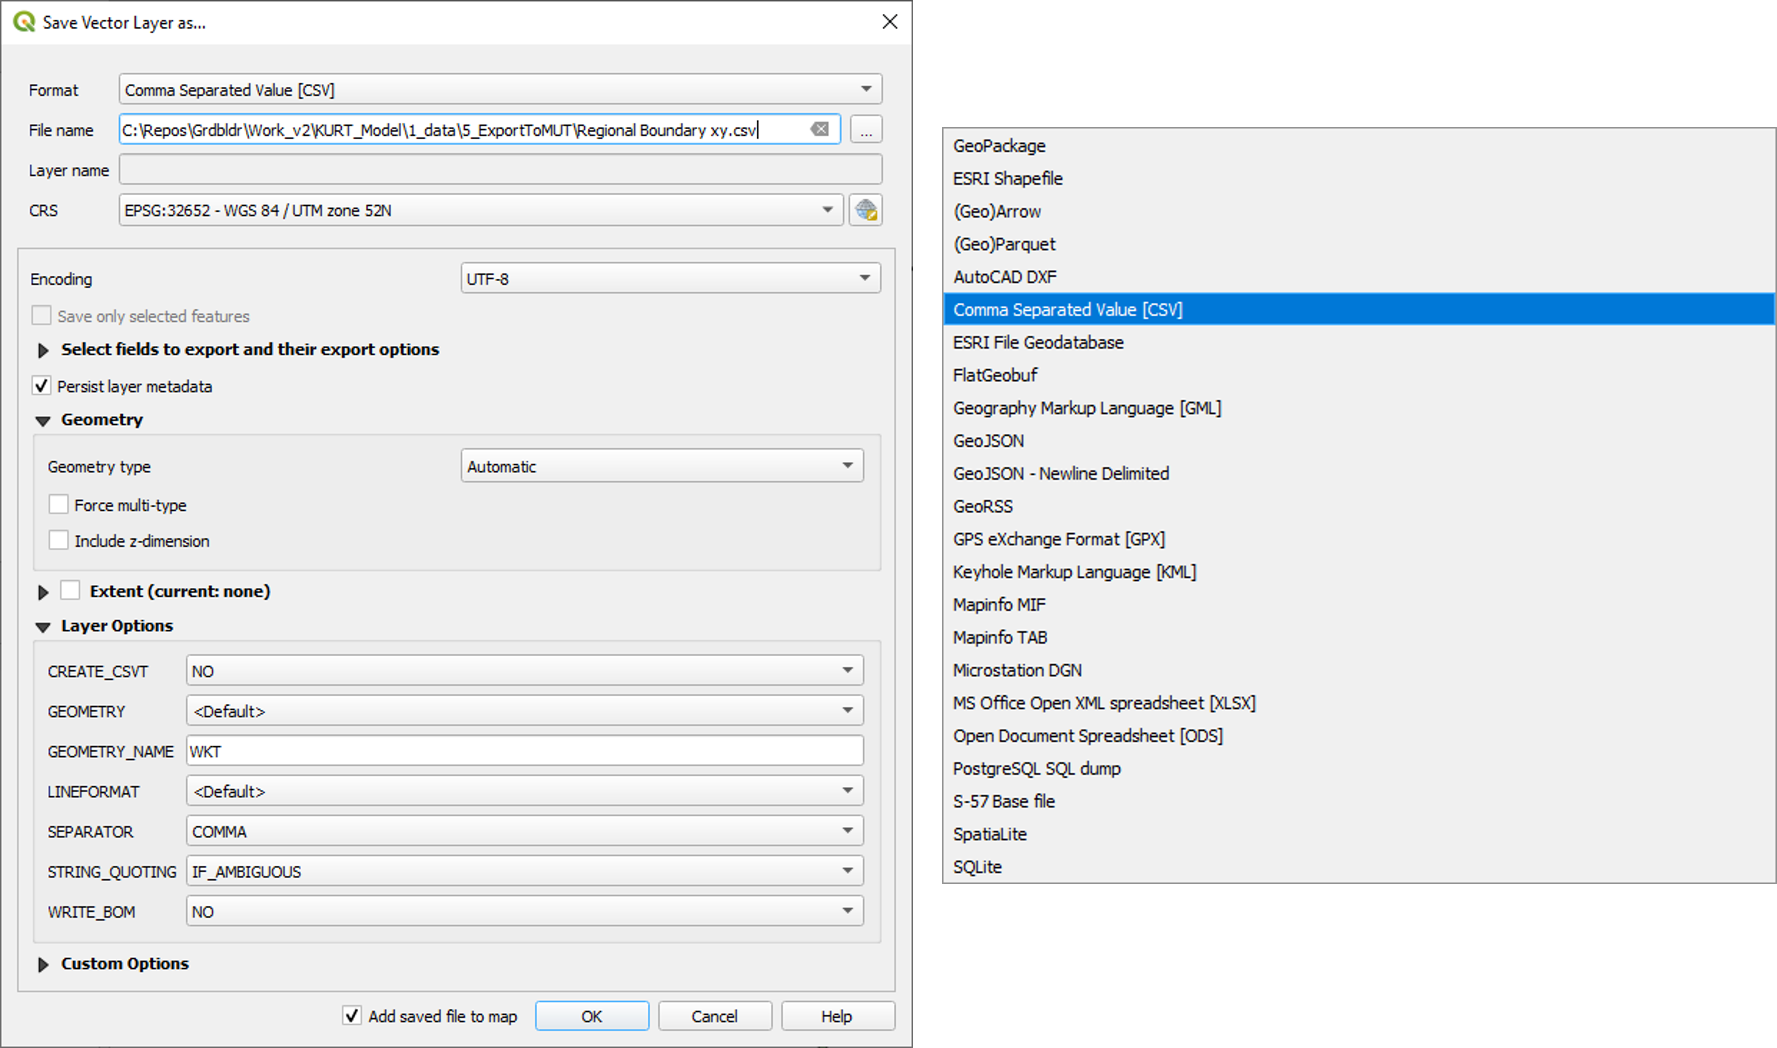
\includegraphics[width=0.9\textwidth]{QGIS_ExportToCSVFile_2.png}

            The {\sf Format} field drop-down menu is shown to the right, with the {\sf Comma Separated Value [CSV]} option highlighted.

            The {\sf File Name} field requires the full path and name of the {\tt CSV} file.  The browse button {\sf ...} at the end of the field is the easiest way to enter the information.

            Check that the {\sf CRS} field is set to the correct coordinate system. Choose {\sf Ok}.

            This creates a new layer whose name is taken from the {\tt CSV} file name, in this example {\sf Regional Boundary xy}.  Right-click on the {\sf Regional Boundary xy} layer and choose {\sf Open Attribute Table} as shown below:

                    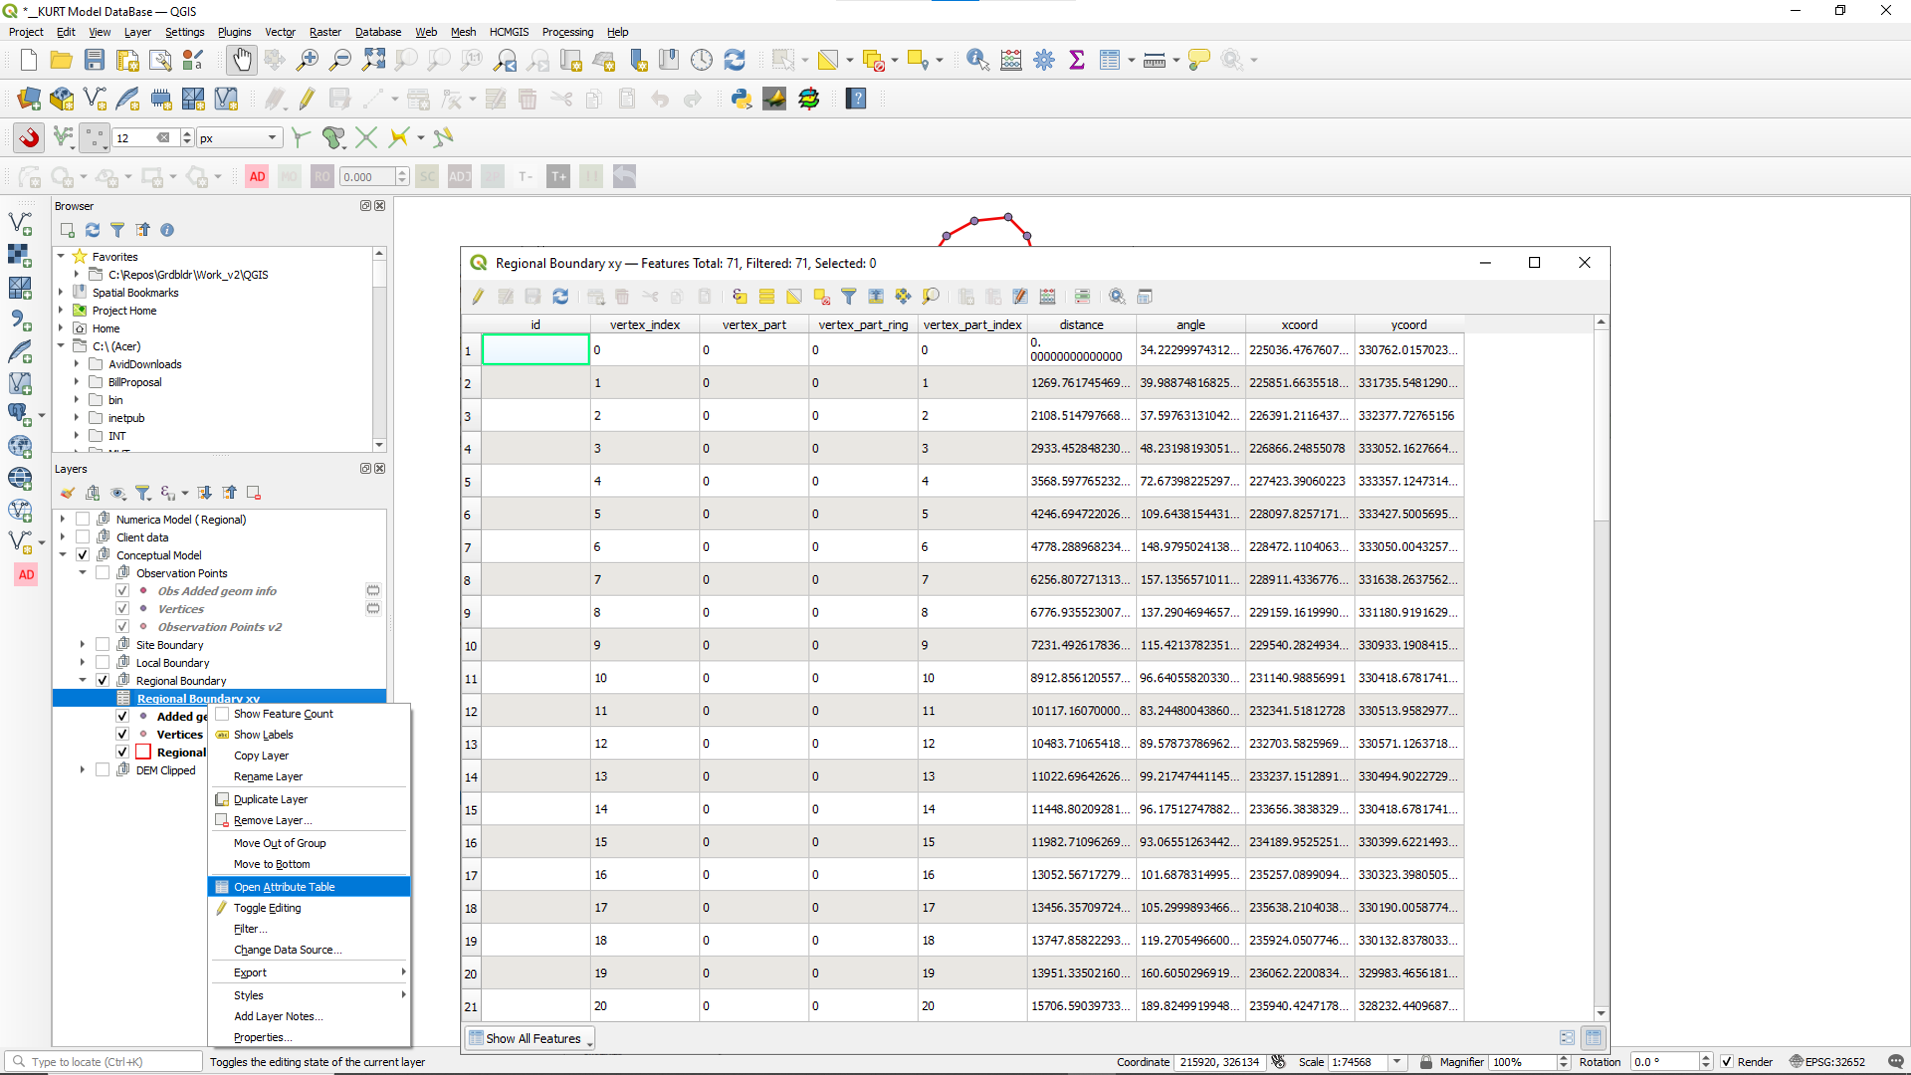
\includegraphics[width=0.9\textwidth]{QGIS_ExportToCSVFile_3.png}


        \newpage
        \subsubsection{Import from a CSV File}
            \label{qgis:ImportFromCSVFile} \index{\qgis\ Usage ! Import from a CSV file}
            A new layer can be created by importing data from a {\tt CSV} file.  Choose \menupath{Layer\Add layer\Add text delimited layer...} as shown below:

                    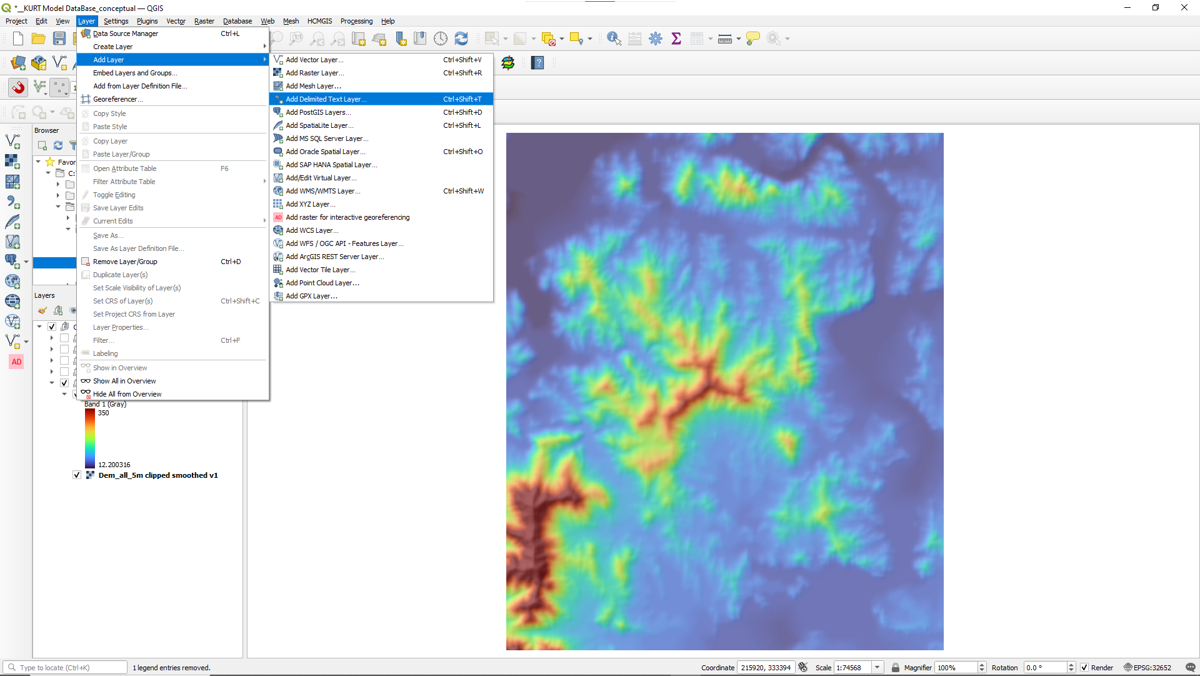
\includegraphics[width=0.9\textwidth]{QGIS_ImportFromCSVFile_1.png}

            This opens the {\sf Delimited Text} dialogue shown below:

                    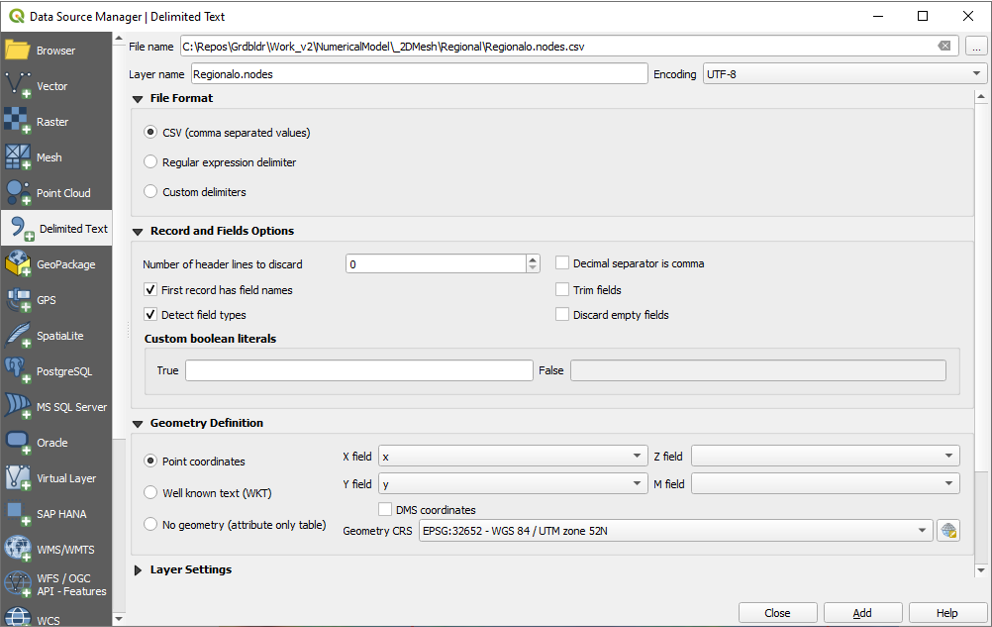
\includegraphics[width=0.6\textwidth]{QGIS_ImportFromCSVFile_2.png}

            The {\sf File Name} field requires the full path and name of the {\tt CSV} file.  The browse button {\sf ...} at the end of the field is the easiest way to enter the information. Choose {\sf Ok}.

            This creates a new layer whose name is taken from the {\tt CSV} file name, in this example {\sf Regionalo.nodes}, and plots the vertices (nodes)as yellow-orange circles shown below:

                    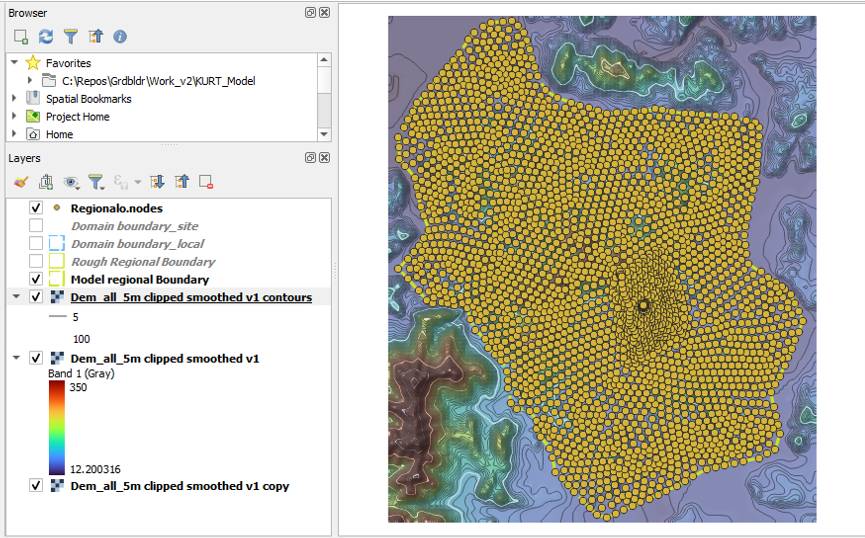
\includegraphics[width=0.9\textwidth]{QGIS_ImportFromCSVFile_3.png}


            Right-click on the {\sf Regionalo.nodes} layer and choose {\sf Open Attribute Table} as shown below:

                    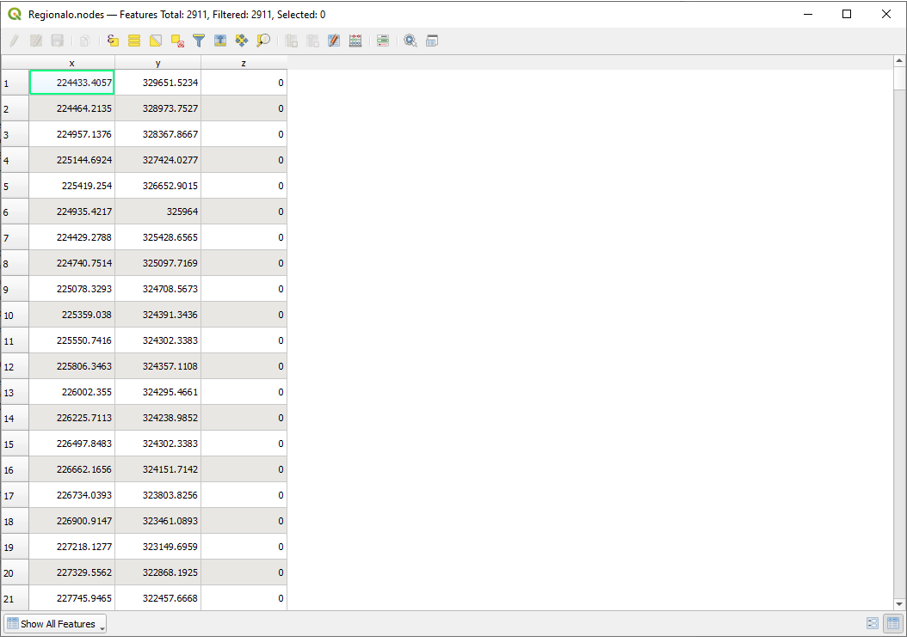
\includegraphics[width=0.9\textwidth]{QGIS_ImportFromCSVFile_4.png}

            This {\tt CSV} file contains a set of $xyz$ coordinates.


    \newpage 
    \subsection{Raster Layers}
        \subsubsection{Loading Raster Layers}
            \label{qgis:LoadRasterLayer} \index{\qgis\ Usage ! Loading a raster layer}
            To load a raster layer, simply drag and drop the raster file into the \qgis\ workspace:

                    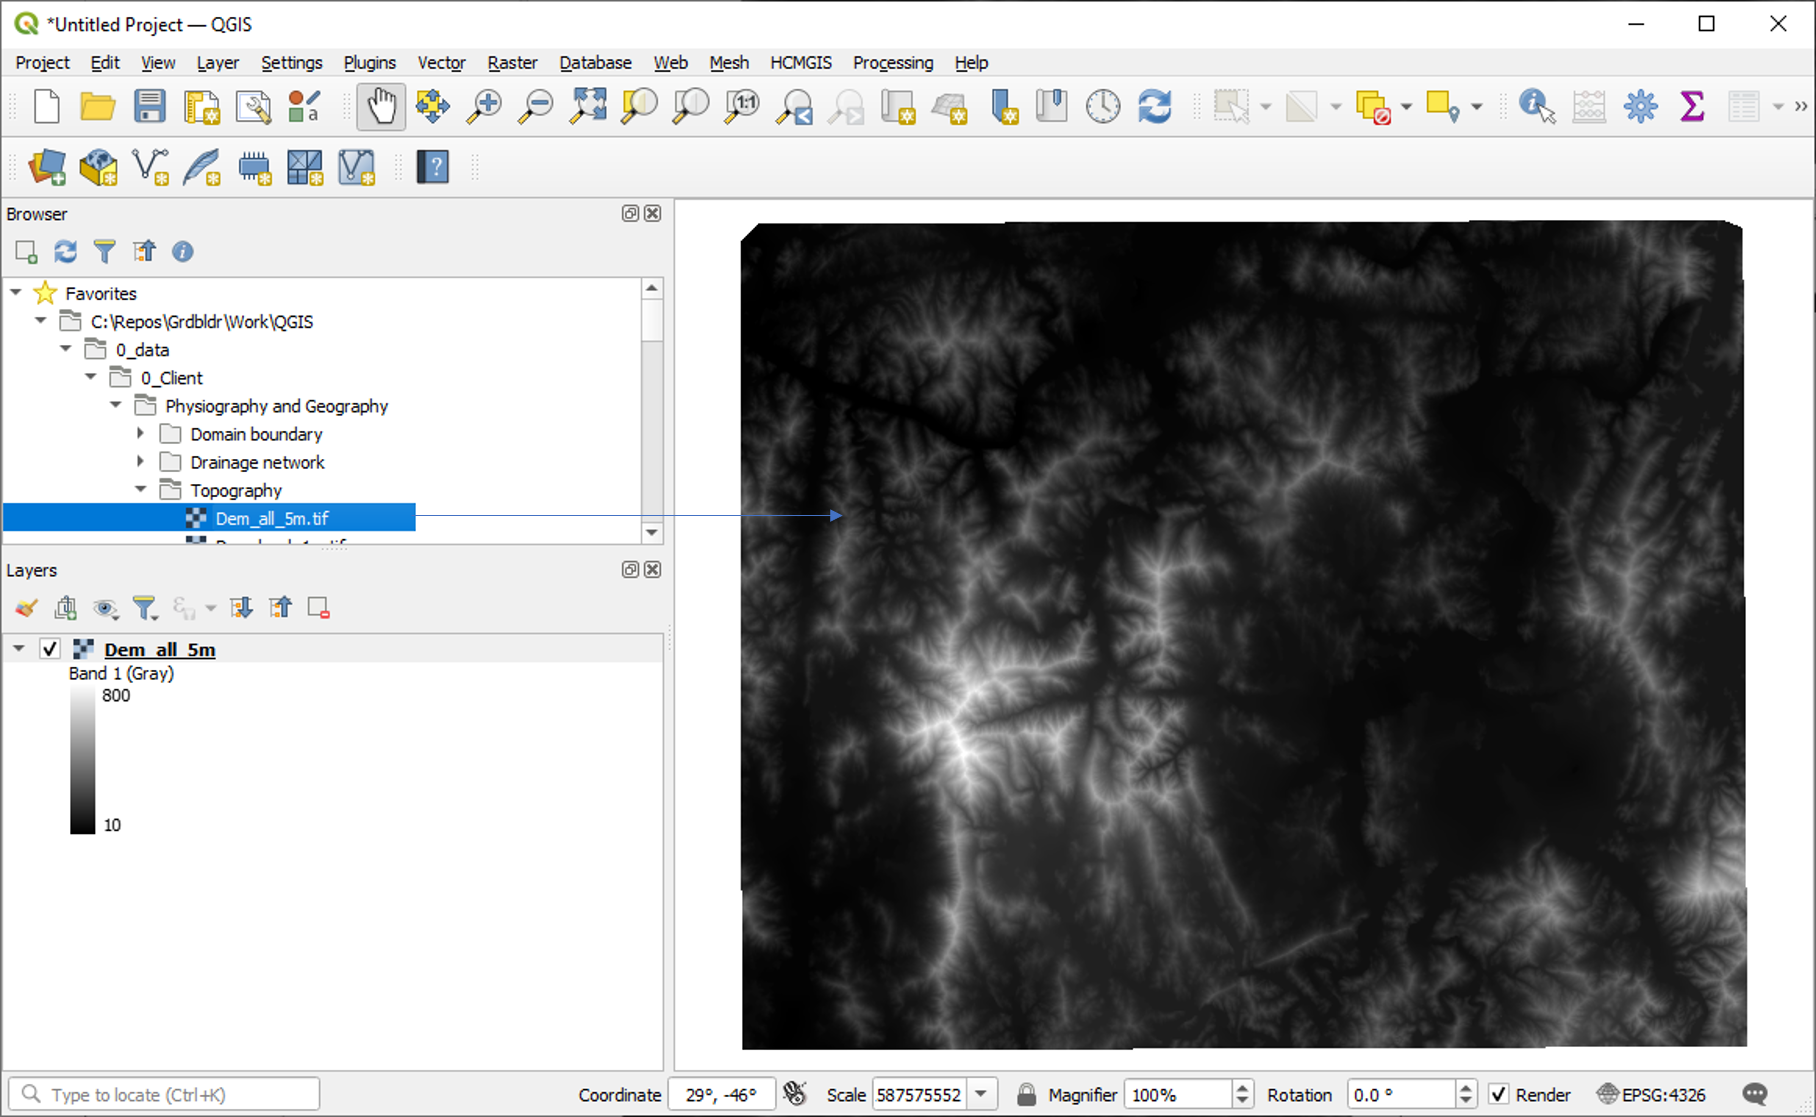
\includegraphics[width=\textwidth]{QGIS_demDrag.png}

            In this example, a raster file \texttt{Dem\_all\_5m.tif} was loaded.  The raster appears in the display with a gray-shading indicating elevation and as an entry in the {\sf Layers} window on the lower left part of the \qgis\ window.  The elevation range (10 to 800 m) and shading scale for the DEM are indicated.

        \newpage
        \subsubsection{Smoothing a Raster Layer}
            \label{qgis:smoothing} \index{\qgis\ Usage ! Smoothing a raster layer}
            A smoothed version a raster layer can be created using the \saga\ plugin \menupath{\Smoothing(ViGrA)}. This plugin must first be installed using \menupath{Plugin\Manage and Install Plugins}, as shown below on the left:

                    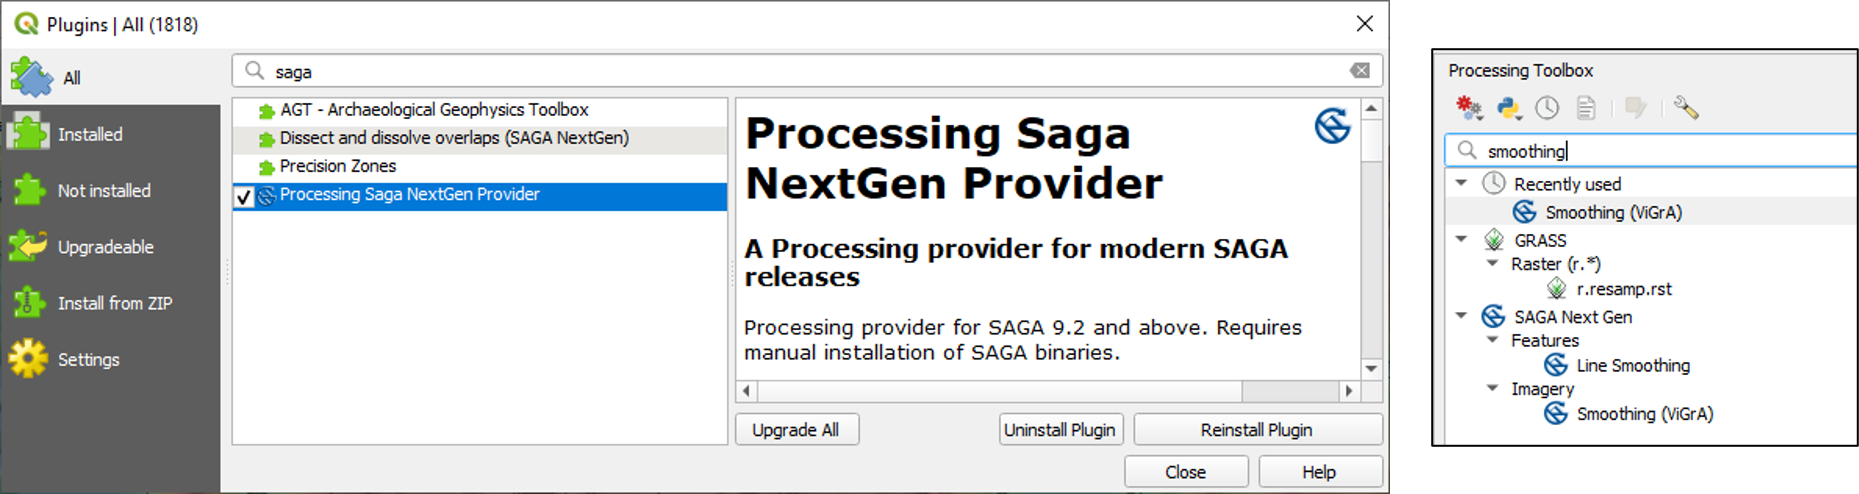
\includegraphics[width=\textwidth]{QGIS_SagaPlugin}

            If the Processing Toolbox panel (above right) is not open choose \menupath{View\Panels\Processing Toolbox}, then search for the string e.g. 'smoothing' to locate the  plugin.

                    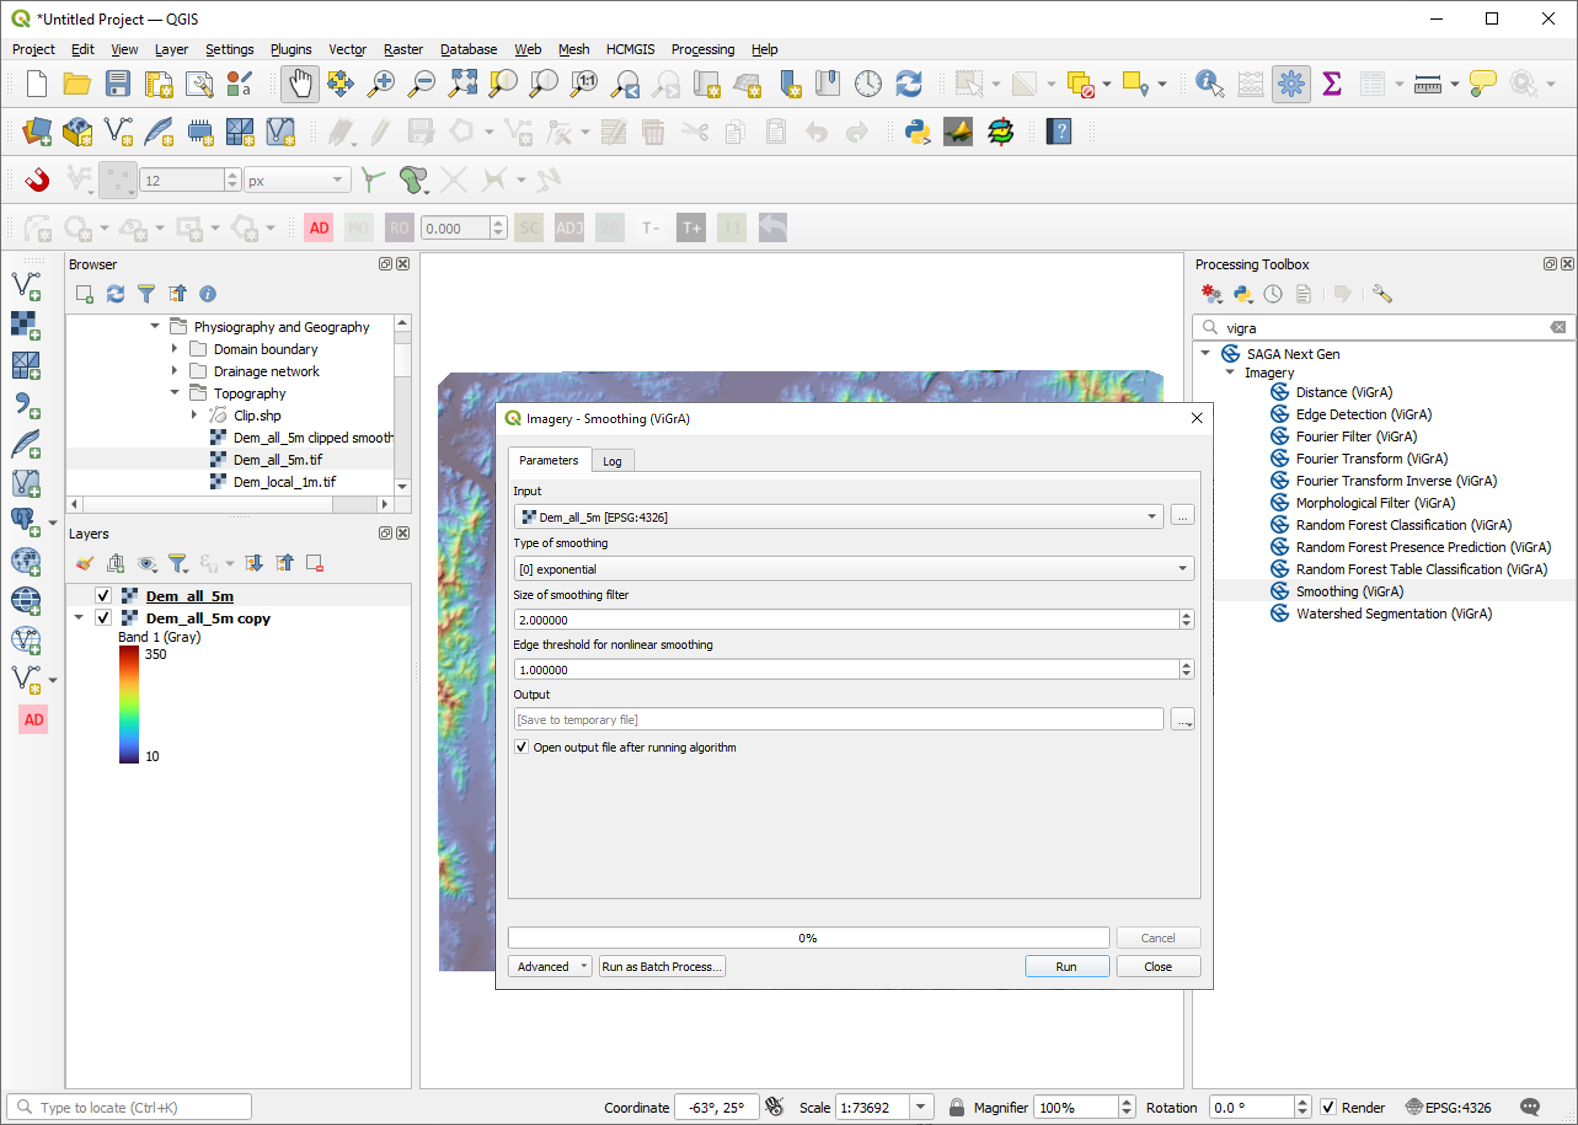
\includegraphics[width=\textwidth]{QGIS_SmoothingDialogue}

            In the example shown above we have chosen to smooth the raster layer {\sf Dem\_all\_5m\_clipped}.  Double-click the {\sf Smoothing(ViGrA)} plugin in to open the dialogue shown below:

            Click the {\sf Run} button to generate a smoothed DEM with a default {\sf Size of smoothing filter} of 2.  The image below shows that a new DEM called {\sf Output} has been created with an elevation range (-9,999 to 792 m).

                    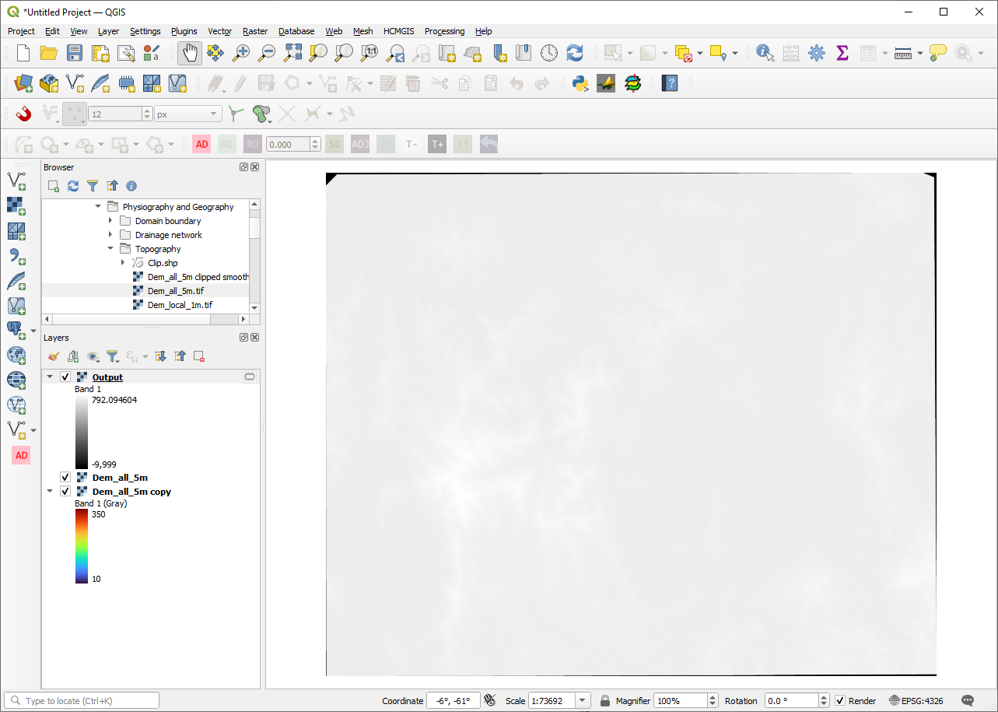
\includegraphics[width=\textwidth]{QGIS_SmoothingDEMInitial.png}


            The regions of -9,999 m elevation show up as black areas around the outside edges of the DEM.  To improve the image choose \menupath{Output\Properties\Symbology} and change the \menupath{Color gradient\Min} value to e.g. 10 m.

            After testing with {\sf Size of smoothing filter} of 2, 5, and 10 m, it was found that the 10 m was sufficient to remove the artefacts.  A portion of the DEM  is shown below both before and after smoothing:

                    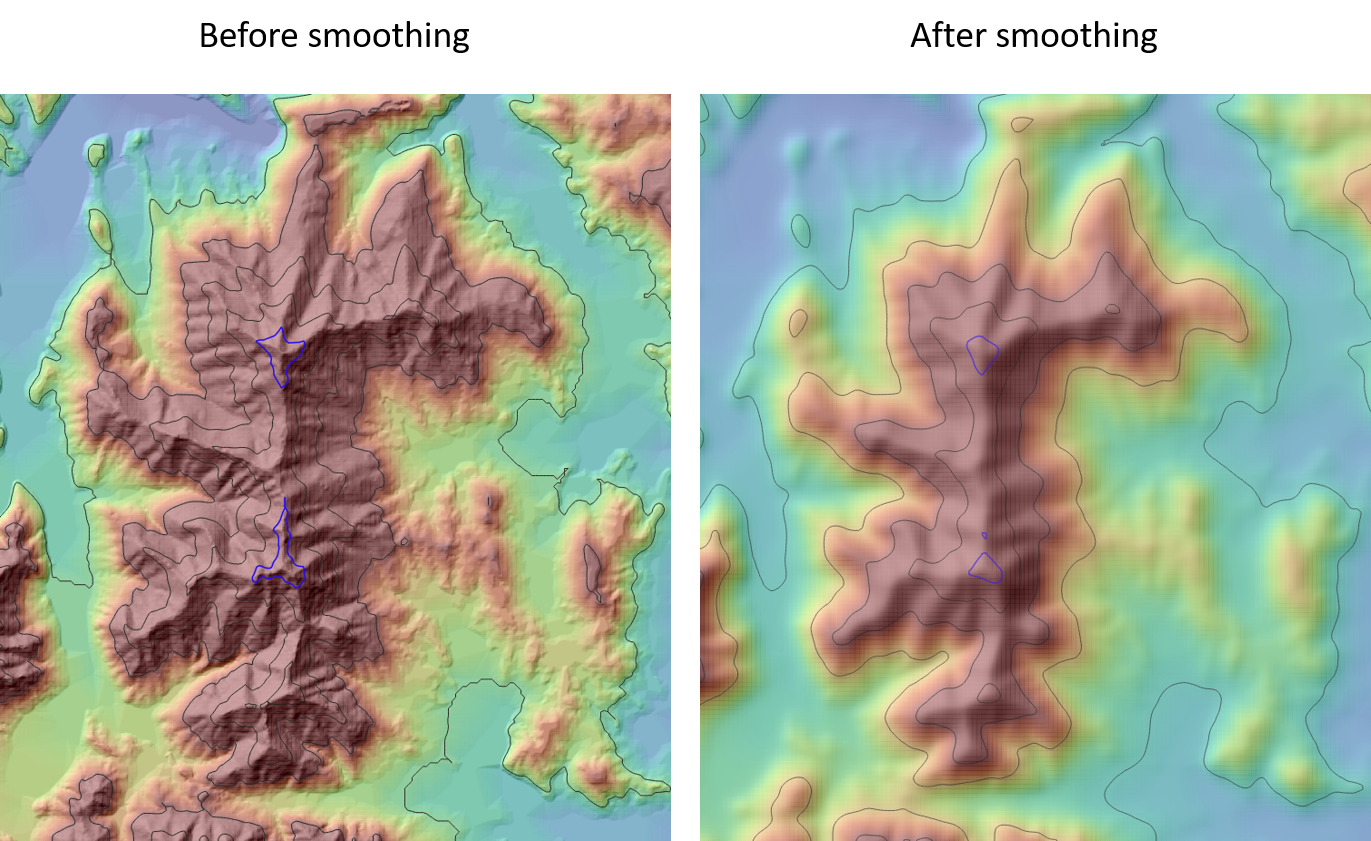
\includegraphics[width=\textwidth]{QGIS_DEMSmoothing.png}


\newpage
\section{Automated Model Set-up}
    \label{qgis:AutomatedSetup} \index{\qgis\ Usage ! Automated model set-up}
    The {\sf MUT Model Builder} \qgis\ plugin automates the first steps of building a hydrogeological model: defining the project and producing the top (ground surface) and bottom (bedrock surface) of the surficial layer for the regional model, then adding high-resolution ground surfaces for focus areas within it.  It can also build a triangular template mesh of the model area for \mut\ (Section~\ref{qgis:MeshGeneration}).  It uses existing project data where it is available and downloads public elevation data where it is not.  The plugin source is in \fpath{MUT_Source\Tools\qgis_mut_builder}.

    \subsection{Installing the Plugin}
        \index{\qgis\ Usage ! MUT Model Builder installation}
        From the \fpath{MUT_Source} folder, run this command in PowerShell:
\begin{verbatim}
.\Tools\qgis_mut_builder\install_plugin.ps1
\end{verbatim}
        This copies the plugin into the default \qgis\ profile as \fpath{mut_model_builder}.  Restart \qgis, then enable {\sf MUT Model Builder} under \menupath{Plugins\Manage and Install Plugins\Installed}.  Run the command again after updating the plugin source.  The command \fpath{install_plugin.ps1 -Remove} removes the installed plugin.

        For plugin development, \fpath{install_plugin.ps1 -Link} links the plugin folder instead of copying it, so source edits take effect when \qgis\ restarts.  Do not uninstall or reinstall a linked plugin from the \qgis\ Plugin Manager: it deletes through the link and removes the plugin source files.  Use \fpath{install_plugin.ps1 -Remove} instead.

    \subsection{Wizard Pages}
        \index{\qgis\ Usage ! MUT Model Builder wizard}
        Choose \menupath{Plugins\MUT Model Builder\New hydrogeological model...} to open the wizard.  It stays open beside the map so you can click on the map while it is open.
        \begin{enumerate}
        \item {\sf Project}: the project name, a free-text description of the hydrogeological system, and an output folder.  {\sf Open existing project.yaml...} reloads a previous project.
        \item {\sf Location}: click {\sf Pick on map} and then the project location, or type its latitude and longitude.  The regional half-width (default 20~km) sets the square model area covered by the $\sim$30~m DEM, outlined in blue.  The model projection defaults to the UTM zone of the location.  {\sf Add OpenStreetMap basemap} helps when the project is empty.  The wizard builds the regional model only; detailed $\sim$1~m surfaces are added afterwards as focus areas (Section~\ref{qgis:FocusAreas}).
        \item {\sf Model boundary}: choose how the model area is defined (see Section~\ref{qgis:ModelBoundary}):
            \begin{itemize}
            \item {\sf Square around the project location}: the regional half-width from the {\sf Location} page (the default).
            \item {\sf Rectangle drawn on the QGIS map}: click {\sf Draw rectangle on map}, then click and drag on the map.
            \item {\sf Watershed found online by name}: type a watershed, basin or river name and click {\sf Search}, or click {\sf Watershed draining to the location}.  Select a result and click {\sf Use selected} (or double-click it).  A river result is delineated at several outlets along the river; the outlines are listed largest first, and you then choose one of them.
            \item {\sf Polygon(s) from a vector file}: a shapefile, GeoPackage, GeoJSON, KML or GML file.  All polygons in the file are merged.
            \end{itemize}
            The chosen boundary is outlined in green and its area is shown.  The regional grid covers the boundary extent plus the margin (default 1~km).  You are warned if the project location lies outside the boundary.
        \item {\sf Existing data}: choose the folder holding existing project data and click {\sf Scan folder}.  Each raster and vector file is listed with a suggested role based on its name and values: {\tt ground\_dem}, {\tt bedrock\_elevation}, {\tt bedrock\_depth\_m}, {\tt bedrock\_depth\_cm}, {\tt bathymetry\_elevation}, {\tt bathymetry\_depth\_m}, {\tt boundary} or {\tt ignore}.  Change any role that is wrong.  Ground DEMs with pixels of 5~m or less are used at full resolution for focus areas and are averaged into the regional surface; coarser ones are used for the regional surface only.  Files named as surface models ({\tt dsm}) are ignored because they include buildings and trees.
        \item {\sf Sources and options}: the download sources that cover the regional area, the optional OpenTopography API key, the regional cell size, the default focus-area cell size (1~m), the minimum surficial thickness (default 1~m), and {\sf Correct lakes with bathymetry} (on by default) with the smallest lake corrected (default 2~ha; Section~\ref{qgis:LakeBathymetry}).  The high-resolution sources are used only when a focus area is built.
        \item {\sf Run}: saves \fpath{project.yaml} and builds the regional surfaces in the background.  When it finishes, the layers are added to the current \qgis\ project and {\sf Open report} shows the run report.  The page shows the size of the regional grid in million cells.  Above 40 million cells you are asked to confirm, with the approximate size of each layer (4 bytes per cell) and the cell size that brings the grid under 40 million cells.  Above 250 million cells the run is refused before anything is downloaded: choose a coarser cell size (up to 1000~m) or draw a smaller boundary.  {\sf Cancel run} also stops a reprojection or download in progress within a few seconds; the partial file is deleted and the log shows {\tt Run canceled}.
        \end{enumerate}

    \subsection{Model Boundary}
        \label{qgis:ModelBoundary} \index{\qgis\ Usage ! MUT Model Builder boundary}
        The boundary is saved as \fpath{<output>\1_data\boundary\model_boundary.geojson} (EPSG:4326), with its name, source and citation stored as attributes.  It is added to the \qgis\ project as the {\sf Model boundary} layer and described in the run report, together with surface statistics for the cells inside it.  The output rasters remain rectangles that cover the boundary plus the margin; the boundary is not used to clip them.

        A watershed search uses these sources:

        \begin{tabular}{p{0.3\textwidth}p{0.62\textwidth}}
        \hline
        Source & Use \\
        \hline
        USGS Watershed Boundary Dataset & Named hydrologic units (HUC2 to HUC12), United States only.  Searched within about 2$^\circ$ of the project location.  The server is sometimes busy; levels that time out are reported and skipped, so search again if the unit you want is missing. \\
        OpenStreetMap & Named rivers, streams and drainage basins worldwide (OpenStreetMap contributors, ODbL). \\
        Global Watersheds & Delineates the area draining to a point from MERIT-Hydro ($\sim$90~m) (Heberger, mghydro.com; Yamazaki et al., 2019).  Used for {\sf Watershed draining to the location}, for river outlets and for focus-area watersheds. \\
        \hline
        \end{tabular}

        \medskip
        Automated delineation can snap an outlet to a tributary or to a neighbouring river at a confluence, so check the green outline against the basemap before running.  {\sf Watershed draining to the location} gives only the small catchment above the location unless it is on the main stream; to get the watershed of a larger river, search for it by name instead.

    \subsection{Data Sources}
        \index{\qgis\ Usage ! MUT Model Builder data sources}
        Local files always take priority.  Download sources are tried in the order below and fill only the cells that are still empty.

        \begin{tabular}{p{0.3\textwidth}p{0.62\textwidth}}
        \hline
        Source & Use and accuracy \\
        \hline
        NRCan MRDEM-30 & Regional ground surface, Canada, no key needed.  Bare-earth model (CGVD2013) built from HRDEM lidar where available, so it matches focus-area lidar closely. \\
        Copernicus GLO-30 & Regional ground surface, worldwide, no key needed.  Accuracy better than 4~m (LE90).  It is a surface model: heights include buildings and forest canopy, so hedgerows, woodlots and roads along survey lines show as bands in a hillshade, and the surface sits a few metres above bare ground. \\
        OpenTopography global DEM & Fallback regional surface (NASADEM, SRTM), 60$^\circ$N to 56$^\circ$S.  Needs a free API key. \\
        USGS 3DEP 1~m & Focus-area surface, United States lidar, about 0.1~m. \\
        NRCan HRDEM & Focus-area surface, Canadian lidar (1--2~m), about 0.1--0.3~m. \\
        AHN (PDOK) & Focus-area surface, Netherlands lidar (0.5~m). \\
        Environment Agency lidar & Focus-area surface, England lidar composite (1~m). \\
        OpenTopography lidar catalogue & Search only: lidar datasets covering the focus area are listed in its report for manual download and processing. \\
        Shangguan et al.\ (2017) & Bedrock, worldwide depth to bedrock at 250~m.  Errors of tens of metres are common; replace with a surface from local boreholes, well logs or geophysics when available. \\
        \hline
        \end{tabular}

        \medskip
        If no high-resolution DEM covers a focus area, its report says so and lists any lidar found in the OpenTopography catalogue.  Put a lidar DEM in the data folder, mark it {\tt ground\_dem} and build the focus area again.

    \subsection{Outputs}
        \index{\qgis\ Usage ! MUT Model Builder outputs}
        All rasters use the model projection and are written to \fpath{<output>\1_data\surfaces}:
        \begin{itemize}
        \item \fpath{ground_top.tif}: the regional ground surface.  Local high-resolution DEMs are averaged to the regional cell size and take priority over downloads.  When lake bathymetry is applied, lakes show the lake bottom (Section~\ref{qgis:LakeBathymetry}).
        \item \fpath{ground_top_water_surface.tif}, \fpath{lake_depth.tif} and \fpath{lakes.geojson}: written only when lake bathymetry is applied; the ground surface before the correction (lake water surfaces), the depth below the water surface, and the corrected lakes.
        \item \fpath{bedrock_bottom.tif}: the bedrock surface.  Depth-to-bedrock data are subtracted from the ground surface.  Bedrock is kept at least the minimum thickness below ground.
        \item \fpath{surficial_thickness.tif}: ground surface minus bedrock surface.
        \item \fpath{sources.json}: where each surface came from, with dates, resolution, vertical accuracy, vertical datum, licence and citation.
        \end{itemize}
        The output folder also holds \fpath{project.yaml}, a run report \fpath{<name>_surfaces_report.md}, and a \qgis\ project \fpath{<name>.qgz} with the styled layers.  Raw downloads are cached in \fpath{<output>\0_incoming\downloads} and reused on later runs.  Focus-area outputs are described in Section~\ref{qgis:FocusAreas}.

    \subsection{Focus Areas}
        \label{qgis:FocusAreas} \index{\qgis\ Usage ! MUT Model Builder focus areas}
        A focus area is a named subregion of a built regional model, for example a wetland and the local watershed that drains to it, with its own $\sim$1~m ground surface.  A project may have any number of focus areas.  Building one does not change the regional surfaces.

        Choose \menupath{Plugins\MUT Model Builder\New focus area...}, then:
        \begin{enumerate}
        \item {\sf Regional project file}: choose the \fpath{project.yaml} of the regional model.  Its regional ground surface must already be built.  If the open \qgis\ project is the plugin's \fpath{<name>.qgz}, its \fpath{project.yaml} is chosen automatically; otherwise the last one used is offered.  The regional grid is outlined in green.
        \item {\sf Focus area name}: type a new name, or pick an existing focus area to review or rebuild it.
        \item Outline the focus area in one of four ways:
            \begin{itemize}
            \item {\sf Rectangle drawn on the map}: click {\sf Draw rectangle on map}, then click and drag.
            \item {\sf Outline digitized on the map}: click {\sf Digitize outline on map}, left-click the vertices, press Backspace to remove the last vertex, and right-click or double-click to close the outline.
            \item {\sf Polygon(s) from a vector file}: all polygons in the file are merged.
            \item {\sf Feature in the regional area}: type a name such as {\tt Luther Marsh} and click {\sf Search}.  OpenStreetMap features inside the regional area are listed, named areas first; the selected one is drawn in grey.  Choose how to outline it and click {\sf Outline selected feature}:
                \begin{itemize}
                \item {\sf Local watershed from the regional ground surface} (the default): flow accumulation and directions are computed from \fpath{ground_top.tif} with GRASS {\tt r.watershed} (once per project, then cached in \fpath{1_data\focus\_hydro}).  The outlet is the cell of largest flow accumulation inside the feature, shown by a blue marker, and {\tt r.water.outlet} gives the watershed draining to it.
                \item {\sf Local watershed from Global Watersheds}: the same outlet is sent to the online Global Watersheds service (MERIT-Hydro, $\sim$90~m).
                \item {\sf Feature outline only}: the feature itself; a point feature becomes a 1~km square.
                \end{itemize}
                The watershed is merged with the feature, because a wetland or lake often extends beyond the watershed of its outlet.
            \end{itemize}
        \item Review the extent.  The outline is drawn in orange and the focus grid (outline extent plus the margin, default 200~m) as a dashed rectangle.  The area, grid size and approximate file size are shown, with a warning above 50 million cells.  Above 50 million cells {\sf Accept extent} and {\sf Download 1 m DEM} ask you to confirm; above 250 million cells they refuse and suggest a coarser cell size or a smaller outline.  Change the {\sf Cell size} (default from the project, normally 1~m) or the margin if needed, or outline the area again.
        \item Click {\sf Accept extent}.  The outline is saved as \fpath{1_data\focus\<name>\focus_boundary.geojson} and the focus area is added to \fpath{project.yaml} with status {\tt defined}.  Nothing large is downloaded yet.
        \item Click {\sf Download 1 m DEM}.  The focus grid is filled from local ground DEMs and the enabled high-resolution sources (Section~\ref{qgis:AutomatedSetup}), in the background with a progress bar and log.  When it finishes, a {\sf \textit{project} focus: \textit{name}} group with the outline, hillshade and ground surface is added to the map, the \qgis\ project \fpath{<name>.qgz} is rewritten to include it, and {\sf Open report} shows the focus report.
        \end{enumerate}

        Each focus area is written to \fpath{<output>\1_data\focus\<name>}:
        \begin{itemize}
        \item \fpath{focus_boundary.geojson}: the accepted outline (EPSG:4326) with its source, feature, delineation method and citation.
        \item \fpath{ground_top_1m.tif} (named for the cell size): the focus-area ground surface.  Small gaps, such as under buildings, are filled.
        \item \fpath{ground_top_1m_hillshade.tif}, \fpath{sources.json} and \fpath{<name>_focus_report.md}.
        \item \fpath{ground_top_1m_water_surface.tif}, \fpath{lake_depth_1m.tif} and \fpath{lakes.geojson}: as for the regional surface, when lake bathymetry is applied.
        \end{itemize}
        The focus dialog has its own {\sf Correct lakes with bathymetry} check box, which is saved as the project option.
        The regional report lists all focus areas with their status.  The focus report gives the outline, outlet, grid, coverage and sources, and the mean difference between the focus DEM (averaged to the regional cell size) and the regional ground surface.  A large offset usually means different vertical datums (e.g.\ EGM2008 for Copernicus and NAVD88 for 3DEP) or a surface model compared with bare ground.

        A watershed delineated from a 30~m surface can be a few cells off in flat wetlands and near drains, and the regional and Global Watersheds outlines may differ by several percent.  Compare the orange outline with the hillshade before accepting it.  A 65~km$^2$ watershed at 1~m is about 130 million cells (500~MB); use a 2~m cell size or a smaller outline when the warning appears.  GRASS is run through \fpath{qgis_process}, which is part of a standard \qgis\ installation.

    \subsection{Lake Bathymetry}
        \label{qgis:LakeBathymetry} \index{\qgis\ Usage ! MUT Model Builder lake bathymetry}
        Lidar DEMs, and the DEMs built from them such as NRCan HRDEM and MRDEM, do not see through water.  Lakes, ponds and reservoirs are hydro-flattened: every cell in a lake has the same elevation, the water surface.  Luther Lake in the Grand River watershed, for example, is a flat surface at 481.6~m.  A groundwater model built on that surface puts the lake bed metres too high.

        With {\sf Correct lakes with bathymetry} on (the default), each lake, pond and reservoir mapped in OpenStreetMap of at least the minimum area (default 2~ha) is lowered to a lake bottom.  Rivers, canals and drains are not changed.  The water level is the median DEM value inside the lake, and the bottom is the water level minus a depth taken, cell by cell, from the first source available:
        \begin{enumerate}
        \item Local files in the data folder with role {\tt bathymetry\_elevation} (lake-bottom elevations) or {\tt bathymetry\_depth\_m} (depth below the water surface, in metres).  Files with {\tt bathy}, {\tt lake bottom} or {\tt sounding} in their name are suggested for these roles.
        \item Measured surveys: Ontario MNRF bathymetry contours and points (Land Information Ontario, Open Government Licence -- Ontario), interpolated within each lake with the shoreline at zero depth.  At least 10 survey samples are needed in a lake.
        \item An estimate, for all other lakes: depth increases linearly with distance from shore (Hollister and Milstead, 2010) to a maximum depth predicted from the median slope of the surrounding land times the largest distance to shore (Hollister et al., 2011).  This is the method used for the GLOBathy global data set (Khazaei et al., 2022).  The minimum maximum depth is 0.5~m.  The estimate needs the whole shoreline, so a lake that extends beyond a focus grid takes its depth from the regional \fpath{lake_depth.tif} (with the regional method), and a lake that extends beyond the regional grid is not corrected.
        \end{enumerate}
        The surface is only ever lowered; cells below the computed bottom are not raised.

        Bathymetry is always reported when it is used:
        \begin{itemize}
        \item The run log shows {\tt Lakes: BATHYMETRY APPLIED to N lake(s)} with the counts by method.
        \item The report has a {\sf Lake bathymetry} section that starts with a bold statement that the ground surface in those lakes is the lake bottom.  A table lists each lake with its area, water level, how flat the DEM was, the depth source (ESTIMATED in capitals), and the maximum and mean depths.  Estimated lakes show the slope and distance used.
        \item The \qgis\ project adds a {\sf Lakes: bathymetry applied} outline layer (estimated lakes dashed magenta, measured blue, local green, not corrected grey), and hidden layers with the lake depth and the ground surface before the correction.  The ground surface layer is named {\sf Ground surface with lake bottoms (bathymetry)}.
        \item \fpath{sources.json} lists the measured and estimated bathymetry as sources, with citations.
        \end{itemize}
        If the lake or survey services cannot be reached, the run continues without the correction and the report says in bold that bathymetry was {\em not} applied.

        Estimated bottoms are not surveys.  Errors of tens of percent are to be expected, and dammed, dredged or marsh lakes do not follow the shape of the land around them.  Ontario surveys are often historic (1950s--1990s) fish-habitat transects, with depths below the water level at the time of the survey.  For a lake that matters to the model, obtain a survey from the conservation authority or lake association and add it with role {\tt bathymetry\_elevation} or {\tt bathymetry\_depth\_m}.

        \textbf{Dams and reservoir levels.}  When bathymetry is applied, the report also has a {\sf Dams and reservoir levels} section listing the dams within 300~m of a corrected lake.  Dams come from the Ontario Dam Inventory (MNRF) in Ontario and from OpenStreetMap elsewhere.  For dams of the Grand River Conservation Authority, the last ten years of hourly measured reservoir elevations are read from the GRCA KiWIS service (provisional data).  The report gives the current, median and 5--95\% range, the monthly medians, and the percentile of the DEM water surface within that record.  This shows whether the lidar was flown at a high or low reservoir level.  Target (rule-curve) elevations are not published as data.  They are read from \fpath{core\data\reservoir_targets.json} in the plugin folder, which holds the values published by GRCA (2016) for the Luther, Shand (Belwood), Conestogo and Guelph dams, each with its citation.  Add entries for other reservoirs in the same form.  Elevations published by a dam owner may use an older vertical datum (e.g.\ CGVD28) than the lidar DEM (CGVD2013).  This step only reports; it does not change the surfaces.

    \subsection{Mesh Generation}
        \label{qgis:MeshGeneration} \index{\qgis\ Usage ! MUT Model Builder mesh generation}
        The plugin can build a 2D Delaunay triangular-element mesh of the model area that \mut\ reads as a template mesh with {\sf 2d mesh from gb} (page~\pageref{texfile:TemplateMesh}).  Combined with {\sf nodal control volumes}, each mesh point becomes a \mf\ cell.  This automates the manual \qgis\ steps (densify and extract boundary vertices, clip regular points, merge, Delaunay triangulation, clip) used for earlier projects.  A regional run is not required; the mesh uses only the model boundary.

        Choose \menupath{Plugins\MUT Model Builder\New mesh...}, then:
        \begin{enumerate}
        \item {\sf Project file}: choose \fpath{project.yaml} (chosen automatically when the plugin's \fpath{<name>.qgz} is open).
        \item {\sf Mesh name}: type a new name, or pick an existing mesh to rebuild it with its saved settings.
        \item {\sf Boundary point spacing} (default 300~m): every vertex of the model boundary, and of any holes, is a mesh point, and sides longer than this spacing get extra points spaced evenly along them.  The outer edges of the mesh therefore lie exactly on the model boundary.  These points are {\em fixed}.
        \item {\sf Boundary simplification} (default 0): a boundary traced from a DEM can have many short sides, each giving small cells.  A positive value removes boundary detail smaller than this distance first; the mesh outline then stays within that distance of the model boundary.  The dialog shows the shortest boundary side, and the log warns when it is less than a tenth of the spacing.
        \item {\sf Interior points} (default 5000): the approximate number of points filling the interior.  They are placed on a hexagonal (equilateral-triangle) lattice whose spacing is adjusted until the count is close to the number requested; points closer than half a spacing to the boundary or to a fixed point are dropped.  The dialog shows the area and the resulting spacing before the mesh is built.  These points are {\em free}.
        \item {\sf Fixed points} (optional): a point layer from the map, or a vector or CSV file (columns {\tt x}/{\tt y}, {\tt xcoord}/{\tt ycoord} or {\tt easting}/{\tt northing}, in the project CRS), for wells, shafts or observation points that must be mesh nodes.  Points outside the boundary are ignored.
        \item {\sf Smoothing passes} (default 0): Laplacian smoothing moves each free point to the mean of its neighbours and triangulates again; fixed points never move.
        \item Click {\sf Build mesh}.  The mesh is built in the background.  When it finishes, a {\sf \textit{project} mesh: \textit{name}} group is added to the map with the triangles and the nodes (fixed red, free blue), and the \qgis\ project is rewritten to include it.
        \end{enumerate}

        Triangles are kept where their centroid lies inside the polygon formed by the boundary points, so concave boundaries and holes are handled.  Every boundary segment is checked; a segment missing from the triangulation is split by a fixed midpoint and the mesh rebuilt.  The log and \fpath{mesh.json} report the largest distance between the mesh outline and the model boundary, the number of nodes (fixed, free, and by source), triangles, the smallest and mean minimum triangle angle, and the element area and side length ranges.  Fixed points very close together give thin triangles; the log warns when this happens.

        Each mesh is written to \fpath{<output>\2_mesh\<name>}:
        \begin{itemize}
        \item \fpath{<name>.grd}, \fpath{.xyc}, \fpath{.in3}, \fpath{.ean}: \gb\ files read by {\sf 2d mesh from gb}.  All elements are in zone 1.
        \item \fpath{<name>.gpkg}: layers {\tt nodes} ({\tt id}, {\tt fixed}, {\tt source}: boundary, interior, user, stream or inserted; {\tt stream\_level}: 0 off the streams) and {\tt elements} ({\tt id}, node numbers {\tt n1}--{\tt n3}, {\tt area}, {\tt min\_angle}), and with streams a {\tt streams} layer ({\tt level}, {\tt name}, {\tt source}, {\tt length\_m}).
        \item \fpath{<name>_xyCoord.csv} ({\tt id}, {\tt xcoord}, {\tt ycoord}, {\tt fixed}, {\tt source}, {\tt stream\_level}) and \fpath{<name>_idNode.csv} ({\tt POINTA}, {\tt POINTB}, {\tt POINTC}, 1-based node numbers).
        \item With streams, \gb\ chosen-node files {\tt <name>.nchos.Stream level }{\em k} (the nodes on level-{\em k} streams) and {\tt <name>.nchos.Streams} (all stream nodes); see Section~\ref{qgis:MeshStreams}.
        \item \fpath{mesh.json}: the settings, statistics and warnings.
        \item \fpath{mut_snippet.txt}: the \mut\ instructions to load the mesh, assuming the model folder is two levels below the project folder (e.g.\ \fpath{<output>\2_models\Regional}):
\begin{verbatim}
nodal control volumes
2d mesh from gb
..\..\2_mesh\<name>\<name>
\end{verbatim}
        \mut\ reads at most 80 characters for the \gb\ prefix, so keep the path relative.
        \end{itemize}
        The {\tt fixed} flag is kept in every output so that later grid relaxation or smoothing can move only the free nodes.

        \subsubsection{Adding Streams}
        \label{qgis:MeshStreams} \index{\qgis\ Usage ! MUT Model Builder mesh streams}
        Check {\sf Add streams} in the {\sf New mesh} dialog to put fixed nodes along the rivers and streams of the model area, with mesh edges following them, so that \swf\ or \cln\ cells and boundary conditions can be assigned along the stream network.  Streams are ranked into {\em levels}: level~1 is the main river (for the Grand River watershed, the Grand River itself), level~2 the streams flowing into a level-1 river (the Nith, Speed, Conestogo, \ldots), level~3 the streams flowing into those, and so on.
        \begin{itemize}
        \item {\sf Source}: {\sf Automatic} tries the Ontario Hydro Network watercourses (Land Information Ontario) inside Ontario, then USGS NHDPlus High Resolution flowlines inside the United States, then OpenStreetMap waterways (rivers and streams) anywhere.  Any of these can be chosen directly.  {\sf From the regional DEM} extracts the streams from the regional ground surface instead (GRASS {\tt r.stream.extract}, after {\tt r.watershed} flow accumulation); it needs a regional run and \qgis\ with GRASS.  Downloads are cached in \fpath{0_incoming\downloads}.
        \item {\sf Levels} (default 2): how many levels to add.
        \item {\sf Minimum stream length} (default 5~km): streams with less than this length inside the boundary are left out.  It also decides how many separate rivers become level~1 in a rectangular model area, where several rivers can enter or leave the area.
        \item {\sf Stream node spacing} (default: the boundary spacing): the distance between nodes along the streams.  Every confluence and every point where a stream crosses the boundary is a node.
        \item {\sf Main river name} (optional): at each confluence, level~1 follows the branch with this name.  Without it, the branch with the most stream length upstream is followed (a stand-in for drainage area); a named branch is preferred while it has at least 30\% of that length.  NHDPlus HR level paths take precedence.
        \item {\sf Include canals}: also use OpenStreetMap canals and NHDPlus HR canals and ditches.
        \item {\sf DEM stream threshold} (default 10~km$^2$): the smallest drainage area that starts a stream when extracting from the DEM.
        \item {\sf Find streams}: downloads (or extracts) and ranks the streams, adds a {\sf \textit{name} streams (preview)} layer styled by level and lists the rivers found at each level, without building the mesh.
        \end{itemize}

        All lines are oriented downstream and joined at shared ends.  A stream that ends within 50~m of another line (a junction without a shared vertex), or within 300~m of the start of another stream whose name does not differ (a stream broken at a pond or culvert), is joined to it.  Where a river splits (braids, side channels), only one downstream branch is kept for the ranking: the one with the same name, or else the longest.  Level-1 rivers are traced upstream from each outlet that lies outside the boundary or within 1~km of it; each stream joining a level-$k$ river is traced the same way and becomes level~$k+1$.  A network that ends well inside the boundary (at a lake, or at a gap in the data) starts at level~2.  The ranked streams are clipped to the boundary.  OpenStreetMap streams are often broken at ponds and lakes, so the official networks give a cleaner ranking where they are available, and Overpass can take several minutes for a large watershed.

        Stream nodes are {\em fixed}.  Nodes of different streams closer than a quarter of the stream spacing are merged (the lower level keeps its position), outlets on the boundary become boundary nodes, and other stream nodes closer than a quarter of the boundary spacing to the boundary are dropped.  Interior points are kept at least half a spacing from the streams.  Every link between consecutive stream nodes is checked after triangulation; a missing link is split by a fixed midpoint, as for the boundary.  The log and \fpath{mesh.json} report the source and its citation, the rivers at each level, the number of stream nodes and how many stream links are mesh edges.  A stream spacing much smaller than the interior spacing gives thin triangles beside the streams; use a few smoothing passes or more interior points.

        The \fpath{.nchos} files have one flag per mesh node, so they are used in the {\tt tmplt} or {\tt swf} active domain (not in a layered \gwf\ domain, which has a node for each layer).  With {\sf nodal control volumes}, {\sf choose cells from gb nodes} chooses the \swf\ cells at the stream nodes; \fpath{mut_snippet.txt} lists the instructions, for example:
\begin{verbatim}
active domain
swf
    clear chosen cells
    choose cells from gb nodes
    ..\..\2_mesh\<name>\<name>.nchos.Stream level 1
    swf constant head
    250.0
\end{verbatim}
        \mut\ reads at most 80 characters for these file names; the log warns when the paths are longer.  Cite the stream source given in \fpath{mesh.json} in model reports.

    \subsection{Running Without the \qgis\ Window}
        \index{\qgis\ Usage ! MUT Model Builder headless}
        The same pipeline runs from a command prompt using the \qgis\ Python environment:
\begin{verbatim}
Tools\qgis_mut_builder.cmd init C:\Work\Site\project.yaml ^
    --name Site --lat 36.42 --lon 127.37 --data C:\Work\Site\0_incoming
Tools\qgis_mut_builder.cmd run C:\Work\Site\project.yaml
\end{verbatim}
        {\tt init} writes \fpath{project.yaml} with suggested data roles, which can be edited before {\tt run}.  By default the boundary is a square of {\tt --regional-km} (default 20) around the project location.  Use one of these options to set the boundary instead:
        \begin{itemize}
        \item {\tt --boundary-rect=W,S,E,N}: a rectangle in decimal degrees.  Keep the {\tt =} when the west longitude is negative.
        \item {\tt --watershed NAME}: a named watershed.  {\tt --pick N} chooses the candidate (default 0); for rivers, {\tt --outlet K} chooses the outlet, largest first.
        \item {\tt --watershed-at-site}: the watershed draining to the project location.
        \item {\tt --boundary-file PATH}: polygons from a vector file.
        \end{itemize}
        {\tt --margin-km} sets the margin (default 1).  With a boundary option, {\tt --lat} and {\tt --lon} may be omitted; the project location is then the boundary centroid.  To see the candidates before choosing, list them:
\begin{verbatim}
Tools\qgis_mut_builder.cmd watersheds "Geum River" --lat 36.42 --lon 127.37
Tools\qgis_mut_builder.cmd watersheds "Geum River" --lat 36.42 --lon 127.37 ^
    --delineate 0
Tools\qgis_mut_builder.cmd init C:\Work\Geum\project.yaml ^
    --name Geum --watershed "Geum River" --pick 0 --outlet 0
\end{verbatim}
        Set the environment variable {\tt OPENTOPOGRAPHY\_API\_KEY} to enable the OpenTopography fallback, and {\tt QGIS\_BIN} if \qgis\ is not installed in \fpath{C:\Program Files\QGIS 3.44.15}.  Add {\tt --refresh} to ignore cached downloads.  {\tt run} and {\tt focus-run} accept {\tt --bathymetry on} or {\tt off} and {\tt --lake-min-ha} to change the lake bathymetry options; both are saved in \fpath{project.yaml}.  {\tt run} and {\tt focus-run} stop with an error before downloading anything when the grid exceeds 250 million cells; add {\tt --allow-large-grid} to run anyway.

        Focus areas (Section~\ref{qgis:FocusAreas}) are defined and built in two steps, so the outline can be checked in \qgis\ before anything large is downloaded:
\begin{verbatim}
Tools\qgis_mut_builder.cmd focus-search C:\Work\GRW\project.yaml "Luther Marsh"
Tools\qgis_mut_builder.cmd focus-add C:\Work\GRW\project.yaml ^
    --name "Luther Marsh" --feature "Luther Marsh" --pick 0 --delineate dem
Tools\qgis_mut_builder.cmd focus-run C:\Work\GRW\project.yaml --name "Luther Marsh"
\end{verbatim}
        {\tt focus-search} lists the features inside the regional area.  {\tt focus-add} saves the outline and prints its area and grid size; give one of {\tt --feature NAME} (with {\tt --pick N} and {\tt --delineate dem}, {\tt global} or {\tt none}), {\tt --rect=W,S,E,N} or {\tt --file PATH}, and optionally {\tt --margin-m} (default 200) and {\tt --res-m} (default: the project's focus-area cell size).  {\tt focus-run} builds the ground surface, writes the focus report and rewrites the \qgis\ project; add {\tt --no-qgz} to skip the \qgis\ project.

        A mesh (Section~\ref{qgis:MeshGeneration}) is built with:
\begin{verbatim}
Tools\qgis_mut_builder.cmd mesh C:\Work\GRW\project.yaml --name Regional ^
    --spacing-m 300 --points 5000 --fixed-points wells.shp --smooth 5
\end{verbatim}
        {\tt --fixed-points}, {\tt --smooth} (default 0) and {\tt --simplify-m} (boundary simplification, default 0) are optional; {\tt --preview} only prints the area, boundary point count and interior spacing, and {\tt --no-qgz} skips rewriting the \qgis\ project.

        Streams (Section~\ref{qgis:MeshStreams}) are added with {\tt --streams auto} (or {\tt ohn}, {\tt nhdplus}, {\tt osm}, {\tt dem}); {\tt streams} only finds and ranks them into \fpath{2_mesh\_streams\<name>_preview.gpkg}:
\begin{verbatim}
Tools\qgis_mut_builder.cmd streams C:\Work\GRW\project.yaml --name Regional ^
    --streams auto --stream-levels 3
Tools\qgis_mut_builder.cmd mesh C:\Work\GRW\project.yaml --name Regional ^
    --spacing-m 300 --points 5000 --streams auto --stream-levels 2 ^
    --main-river "Grand River"
\end{verbatim}
        The other stream options are {\tt --stream-min-km} (default 5), {\tt --stream-spacing-m} (default: the boundary spacing), {\tt --canals} and {\tt --dem-threshold-km2} (default 10); {\tt streams} also accepts {\tt --refresh}.




